% ======================================================================
%  The analytic reduction in Alpoge's formal proof of the
%  Generalized Riemann Hypothesis
%  Ishaan Dixit
%  Single file; compiles with two runs of pdflatex (TeX Live 2023 or later).
%  License: CC BY 4.0.
% ======================================================================
\documentclass[11pt]{amsart}

\usepackage[utf8]{inputenc}
\usepackage[T1]{fontenc}
\usepackage{lmodern}
\usepackage[margin=1.1in]{geometry}
\usepackage{amsmath,amssymb,amsthm,mathtools}
\usepackage{booktabs,longtable,array}
\usepackage{enumitem}
\usepackage{tikz}
\usetikzlibrary{arrows.meta,positioning}
\usepackage[hidelinks]{hyperref}
\usepackage{url}
\setlength{\emergencystretch}{3em}

% Lean identifiers (used only in remarks and the appendix)
\urlstyle{tt}
\DeclareUrlCommand\lean{\urlstyle{tt}}
\makeatletter\g@addto@macro{\UrlBreaks}{\do\_\do\a\do\e\do\i\do\o\do\u\do\r\do\n\do\t\do\s}\mathchardef\UrlBreakPenalty=9000\makeatother

\newcommand{\CC}{\mathbb{C}}
\newcommand{\R}{\mathbb{R}}
\newcommand{\Z}{\mathbb{Z}}
\newcommand{\N}{\mathbb{N}}
\newcommand{\Q}{\mathbb{Q}}
\newcommand{\eps}{\varepsilon}
\newcommand{\re}{\operatorname{Re}}
\newcommand{\im}{\operatorname{Im}}
\newcommand{\gE}{\gamma_{E}}
\newcommand{\ASK}{\mathrm{ASK}}
\newcommand{\MAIN}{\mathrm{MAIN}}
\newcommand{\De}{\mathrm{De}}
\newcommand{\Th}{\mathrm{Th}}
\newcommand{\Gh}{\widehat{G}}
\newcommand{\pa}{\pi}
\newcommand{\pos}[1]{\left(#1\right)_{+}}
\newcommand{\abs}[1]{\left|#1\right|}
\newcommand{\norm}[1]{\left\|#1\right\|}
\newcommand{\Ga}{\Gamma}
\newcommand{\Oc}{\mathcal{O}}
\DeclareMathOperator{\rk}{rk}

\theoremstyle{plain}
\newtheorem{theorem}{Theorem}[section]
\newtheorem{proposition}[theorem]{Proposition}
\newtheorem{lemma}[theorem]{Lemma}
\newtheorem{corollary}[theorem]{Corollary}
\newtheorem*{theoremA}{Theorem A}
\newtheorem*{theoremB}{Theorem B}
\newtheorem*{theoremC}{Theorem C}
\newtheorem*{maincor}{Corollary (GRH for Dirichlet $L$-functions)}
\theoremstyle{definition}
\newtheorem{definition}[theorem]{Definition}
\newtheorem{remark}[theorem]{Remark}
\newtheorem{example}[theorem]{Example}

\numberwithin{equation}{section}
\setlist{itemsep=2pt,topsep=4pt}

\begin{document}

\title[The analytic reduction in Alp\"oge's proof of GRH]{The analytic reduction in Alp\"oge's formal proof\\ of the Generalized Riemann Hypothesis}

\author{Ishaan Dixit}
\address{Arizona State University, Tempe, AZ 85281, USA}
\email{idixit@asu.edu}

\date{23 November 2026}

\subjclass[2020]{Primary 11M26; Secondary 11N05, 11R23, 68V15}
\keywords{Generalized Riemann Hypothesis, Dirichlet $L$-functions, Landau's theorem, formal proof, Lean}

\begin{abstract}
In November 2026 L.~Alp\"oge released a Lean~4 development, accepted by the Lean kernel and by
several independent checkers, whose final theorem states that no Dirichlet $L$-function vanishes
in $\re s>1/2$. It comes with no human-readable proof. We give conventional proofs of the
analytic part of the argument and of several layers of the arithmetic part, and an exact statement
of what remains.

The analytic part has two theorems. The first is a windowed Landau theorem: a one-sided bound
$G(y)\le Cy^\theta$ for a positive combination of Chebyshev remainders, required only on windows
$[Y,Y^{1+\delta}]$ with $Y$ arbitrarily large, excludes zeros with $\re s>\theta$. No positivity of
Dirichlet coefficients is used. The second reduces such a bound to an averaged inequality between a
weighted count of prime powers and an explicit main term, on a finite abelian group with Frobenius
and inertia data. The admissible error is of size $x/m+m$ for a free integer $m$, and taking
$m\approx\sqrt x$ is the source of the exponent $1/2$.

The averaged inequality in turn follows from eleven conditions (S0)--(S10) (a domain condition
and ten inequalities) between slopes and heights of a family of Hermitian lattices. We prove this
deduction, and we prove the general statements behind four of the ten: a frame theorem for nearly
orthogonal families of Hermitian lattices, a summation of local indices, a congruence modulo
$\sqrt p$, and a divisor inequality for lattices given by local data. The existence of lattices
satisfying the eleven conditions is certified by the Lean kernel and stated precisely, but not
reproved.
\end{abstract}

\maketitle

\setcounter{tocdepth}{1}
\tableofcontents
% ======================================================================
\section{Introduction}\label{sec:intro}
% ======================================================================

\subsection{The result}

On 20 November 2026 Levent Alp\"oge released a formal development in Lean~4~\cite{lean4}, built on
Mathlib~\cite{mathlib}, with a four-page outline~\cite{alpoge-remark}. Its final theorems state:

\begin{maincor}
For every Dirichlet character $\chi$ and every $s\in\CC$ with $\re s>1/2$ (and $s\neq 1$ if $\chi$ is principal),
$L(s,\chi)\neq 0$. In particular every zero of $\zeta$ other than $-2,-4,-6,\dots$ has real part $1/2$.
\end{maincor}

The development has $175{,}187$ files and about $17.4$ million lines. It is accepted by the Lean
kernel and by the independent checkers \texttt{nanoda}, \texttt{con-leche} and \texttt{lean4lean},
among others~\cite{sutherland}, and uses only the axioms \texttt{propext}, \texttt{Quot.sound} and
\texttt{Classical.choice}. The author rebuilt it and re-exported the kernel declarations of the
final theorem; the export agrees byte for byte with the published one~\cite{dixit-repo}.

The outline is four pages and the formal proof has about a million declarations. This paper gives
conventional proofs of as much of the argument as we can, and states the rest exactly.

\subsection{The three theorems}

Throughout, $\Lambda$ is the von Mangoldt function, $\gE$ is Euler's constant and
$(u)_+=\max(u,0)$. For a Dirichlet character $\chi$ which is either nonprincipal or the trivial
character of modulus $1$ we put
\begin{equation}\label{eq:Gchi}
G_\chi(y)=
\begin{cases}
\displaystyle\sum_{n\le y}\Lambda(n)\Bigl(\frac yn-1\Bigr)-y\log y+(1+\gE)\,y, & \chi=1 \text{ of modulus } 1,\\[10pt]
\displaystyle\sum_{n\le y}\Lambda(n)\chi(n)\Bigl(\frac yn-1\Bigr)+y\,\frac{L'(1,\chi)}{L(1,\chi)}, & \chi \text{ nonprincipal}.
\end{cases}
\end{equation}
The sum $\sum_{n\le y}\Lambda(n)\chi(n)(y/n-1)=\int_1^y\psi(t,\chi)\,dt/t$ is a logarithmic
Riesz mean of the Chebyshev function, and $G_\chi$ is what is left after its main term is removed.
For $\chi=1$ we write $G_\zeta=G_1$. The Riemann Hypothesis is equivalent to
$G_\zeta(y)=O(y^{1/2+\eps})$ for every $\eps>0$.

A \emph{character family} $F$ is a finite collection of such characters $\chi_i$ with weights
$a_i>0$, and we put $G_F(y)=\sum_i a_i\re G_{\chi_i}(y)$.

\begin{theoremA}[Windowed Landau theorem; Theorem~\ref{thm:A}]
Let $F$ be a character family, $0<\theta<1$, $\delta>0$ and $C\in\R$. Suppose that for every $Y_0$
there is $Y\ge Y_0$ such that
\[
G_F(y)\le C\,y^{\theta}\qquad\text{for all } y\in[Y,Y^{1+\delta}].
\]
Then $L(s,\chi_i)\neq 0$ for every $i$ and every $s$ with $\re s>\theta$.
\end{theoremA}

Landau's classical theorem gives the same conclusion from a bound valid for all large $y$, and
its usual proof uses that the Dirichlet coefficients of the combined series are nonnegative. In
Theorem~A the bound is needed only on a sequence of windows whose logarithmic length tends to
infinity, and the coefficients $\Lambda(n)\sum_ia_i\re\chi_i(n)$ may have either sign. The
positivity that the proof uses is that of the residues at real poles; see
Remark~\ref{rem:nopositivity}.

Theorem~B produces the hypothesis of Theorem~A. It is formulated on a finite abelian group
$G=(\Z/2\Z)^2\times H$ equipped with data that imitate the Frobenius elements and inertia groups of
an abelian extension of $\Q$ (Definition~\ref{def:datum}). These data turn every character $\psi$
of $G$ into an arithmetic function $\psi_D$ and hence into a function $G_\psi$ of the shape
\eqref{eq:Gchi}. Out of them we build two explicit quantities attached to a scale $a>0$, a point
$t\in H$ and positive weights $w$ (Definition~\ref{def:ask}). The first, $\ASK(a,t,w)$, is a
weighted count of prime powers $p^i<a/w$ at primes inert in a quadratic subextension. The
second, $\MAIN(a,w)$, has the shape of a Stirling main term plus a logarithmic derivative at $s=1$.

\begin{theoremB}[Isolation and balance; Theorem~\ref{thm:B}]
Suppose that at a scale $x$ an abstract host carries $m$ systems of weights, indexed by
$j=1,\dots,m$. Suppose the weights satisfy size conditions, auxiliary characters satisfy
standard bounds, and the averaged inequality
\begin{multline*}
\sum_{t\in T}\sum_{j=1}^{m}\Bigl(\ASK(a_t,t,w_{u,j})-\re\MAIN(a_t,w_{u,j})\Bigr)\\
\le\ x^{C\eps}\Bigl(n_T\,a_E\Bigl(1+\frac{m^2}{k}\Bigr)+m\Bigl(2nmb\,x^{\eps}+\frac{n_{T_2}\,k\,b\,x^{2\eps}}{n^{2}}\Bigr)\Bigr)
\end{multline*}
holds for every translate $u$ in a subgroup $A_0\le H$. Then a weighted sum of the $G_\psi(x)$ over a
prescribed set of characters is at most $x^{1/2+(C+3)\eps}$, plus the absolute values of the
remaining $G_\psi(x)$.
\end{theoremB}

The precise hypotheses are (B0) to (B8) in Section~\ref{sec:B}. They involve only finite
Fourier analysis, Mertens' estimate and Chebyshev's bound, and so does the proof. Relative to the
main term $n_T\,m\,b$, the error bracket is about $x/m+m$ (Section~\ref{sec:balance}). With
$m\approx\sqrt x$ both terms are $\sqrt x$, and this is the only place in the argument where the
exponent $1/2$ is produced.

\begin{theoremC}[Existence of hosts; Theorem~\ref{thm:C}]
For every primitive Dirichlet character $\psi$ there are constants such that, for every
sufficiently small $\eps>0$ and every large $x$ in a set containing windows $[Y,Y^{3/2}]$ with $Y$
arbitrarily large, there is a host satisfying the hypotheses of Theorem~B whose kept characters
are the characters of the cyclic group generated by $\psi$.
\end{theoremC}

Theorem~C is not reproved here. Its formal proof goes through a further layer that we do prove:
the averaged inequality follows from eleven conditions (S0)--(S10) (a domain condition and ten
inequalities) between slopes and heights of a family of Hermitian lattices attached to the host
(Theorem~C1, Section~\ref{sec:slope}). What is left is the existence of such lattices (Theorem~C2,
Section~\ref{sec:C}). For four of the ten inequalities we prove the general statement behind them
and isolate what is specific to the family: the frame inequality (S8), the local indices (S6) and
the losses (S7) in Section~\ref{sec:three}, and the divisibility inequality (S1) in
Section~\ref{sec:S1}.

\subsection{Scope}

Everything outside Theorem~C2 is proved here. The external inputs are standard facts about
Dirichlet $L$-functions ((F1)--(F5) in Section~\ref{sec:prelim}), standard facts about
Harder--Narasimhan filtrations (Section~\ref{sec:three}), and the product formula and
elementary-divisor theory over $\Oc_K$ (Section~\ref{sec:S1}). Theorem~C2 is used as a black box,
and we say so where it is used.

The proofs follow the formal ones but are written independently and in a different order. Every
statement has been compared with its formal counterpart in the published archive (commit
\texttt{40e56bab}); Appendix~\ref{app:lean} gives the correspondence. Where we simplify a formal
statement, we say so.

The mathematics is Alp\"oge's. As written statements, the following appear to be new: the
windowed Landau theorem without positivity of coefficients (Theorem~A); the interface between the
analytic and arithmetic parts as a single averaged inequality (Theorem~B); the analysis of the
error bracket, which shows that a per-lift cost growing linearly along the chain would give the
exponent $2/3$ of the outline (Section~\ref{sec:balance}); and the general forms of the frame,
local-index and divisor inequalities (Sections~\ref{sec:three} and~\ref{sec:S1}). An informal
account of the whole development is~\cite{dixit-account}; see also~\cite{naskrecki,jaswal}.

\subsection{Organization}

Section~\ref{sec:prelim} collects classical facts. Section~\ref{sec:A} proves Theorem~A.
Sections~\ref{sec:hosts}--\ref{sec:balance} introduce hosts, prove Theorem~B and analyse the error.
Section~\ref{sec:slope} proves Theorem~C1, and Section~\ref{sec:C} states Theorems~C and~C2.
Sections~\ref{sec:three} and~\ref{sec:S1} prove the general statements behind (S1), (S6), (S7) and
(S8). Section~\ref{sec:GRH} deduces the Corollary, and Section~\ref{sec:remarks} lists what remains.

\begin{figure}[ht]
\centering
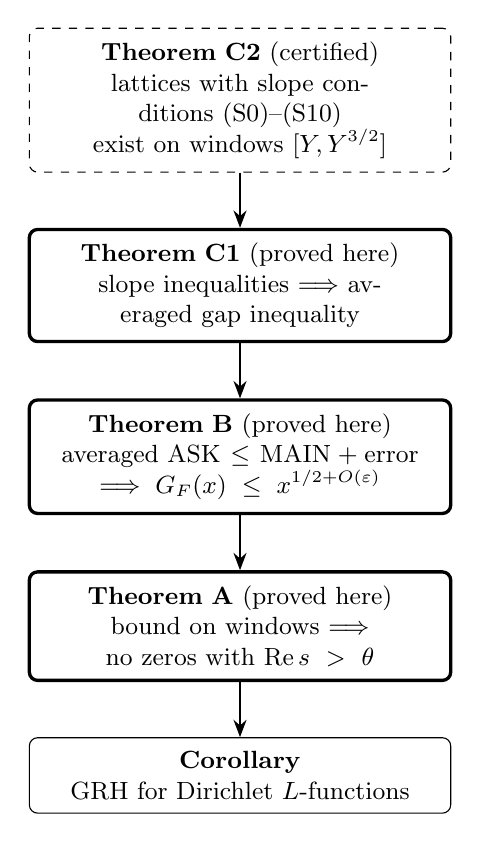
\begin{tikzpicture}[
  box/.style={draw, rounded corners=3pt, align=center, font=\small, inner sep=5pt, text width=50mm},
  bbox/.style={box, draw=black, very thick},
  gbox/.style={box, dashed},
  arr/.style={-{Stealth[length=2.2mm]}, thick}]
\node[gbox] (C2) {\textbf{Theorem C2} (certified)\\ lattices with slope conditions (S0)--(S10)\\ exist on windows $[Y,Y^{3/2}]$};
\node[bbox, below=7mm of C2] (C) {\textbf{Theorem C1} (proved here)\\ slope inequalities $\Longrightarrow$ averaged gap inequality};
\node[bbox, below=7mm of C] (B) {\textbf{Theorem B} (proved here)\\ averaged $\ASK\le\MAIN+\text{error}$\\ $\Longrightarrow G_F(x)\le x^{1/2+O(\eps)}$};
\node[bbox, below=7mm of B] (A) {\textbf{Theorem A} (proved here)\\ bound on windows $\Longrightarrow$ no zeros with $\re s>\theta$};
\node[box, below=7mm of A] (G) {\textbf{Corollary}\\ GRH for Dirichlet $L$-functions};
\draw[arr] (C2) -- (C); \draw[arr] (C) -- (B); \draw[arr] (B) -- (A); \draw[arr] (A) -- (G);
\end{tikzpicture}
\caption{Logical structure. Solid boxes are proved in this paper; the dashed box is a statement
certified by the Lean kernel and not proved here.}\label{fig:structure}
\end{figure}
% ======================================================================
\section{Preliminaries}\label{sec:prelim}
% ======================================================================

\subsection{Characters and classical facts}

A Dirichlet character is \emph{admissible} if it is nonprincipal, or if it is the trivial
character of modulus $1$. For admissible $\chi$ the function $G_\chi$ is defined by
\eqref{eq:Gchi}, and $\bar\chi$ denotes the complex conjugate character, which is again
admissible. We write
\[
R_\chi(y)=\sum_{n\le y}\Lambda(n)\chi(n)\Bigl(\frac yn-1\Bigr)=\sum_{n\ge1}\Lambda(n)\chi(n)\Bigl(\frac yn-1\Bigr)_{+}
\qquad(y\ge0),
\]
so that $G_\zeta(y)=R_1(y)-y\log y+(1+\gE)y$ and $G_\chi(y)=R_\chi(y)+y\,L'(1,\chi)/L(1,\chi)$ for
nonprincipal $\chi$. We use the following standard facts.

\begin{enumerate}[label=\textbf{(F\arabic*)}, leftmargin=3.2em]
\item\label{F1} (Mertens) There is an absolute constant $C_M\ge1$ such that
  $\bigl|\sum_{n\le y}\Lambda(n)/n-\log y\bigr|\le C_M$ for all $y\ge1$; see
  \cite[Section~2.2]{montgomery-vaughan}.
\item\label{F2} (Chebyshev) $\sum_{n\le y}\Lambda(n)\le 2y$ for all $y>0$. This follows from
  $\psi(y)<1.04\,y$ \cite[Theorem~12]{rosser-schoenfeld}.
\item\label{F3} For nonprincipal $\chi$, $L(s,\chi)$ extends to an entire function; $(s-1)\zeta(s)$
  extends to an entire function, and $\zeta(s)=\frac1{s-1}+\gE+O(s-1)$ near $s=1$. For
  $\re s>1$, $-\frac{L'}{L}(s,\chi)=\sum_{n\ge1}\Lambda(n)\chi(n)n^{-s}$, with absolute convergence.
  Moreover $\overline{L(\bar s,\chi)}=L(s,\bar\chi)$. See \cite[Chapter~10]{montgomery-vaughan} and
  \cite{davenport}.
\item\label{F4} $L(s,\chi)\neq0$ for $\re s\ge1$ and nonprincipal $\chi$, and $\zeta(s)\neq0$ for
  $\re s\ge1$; see \cite[Chapters~6 and~11]{montgomery-vaughan} and \cite{davenport}.
\item\label{F5} The zeros of an entire function that is not identically zero are isolated and of
  finite order.
\end{enumerate}

By \ref{F3} the constant $L'(1,\chi)/L(1,\chi)$ in \eqref{eq:Gchi} is well defined, since
$L(1,\chi)\neq0$ by \ref{F4}. Complex conjugation gives
\begin{equation}\label{eq:conj}
\overline{G_\chi(y)}=G_{\bar\chi}(y),\qquad \re G_\chi(y)=\tfrac12\bigl(G_\chi(y)+G_{\bar\chi}(y)\bigr).
\end{equation}

\begin{lemma}\label{lem:growth}
For every admissible $\chi$ there is $C_\chi$ with $|G_\chi(y)|\le C_\chi\,y^{2}$ for all $y\ge1$.
\end{lemma}

\begin{proof}
By \ref{F1}, $|R_\chi(y)|\le y\sum_{n\le y}\Lambda(n)/n\le y(\log y+C_M)$. Also $y\log y\le y^2$,
and the remaining terms are $O(y)$.
\end{proof}

\subsection{The Mellin transform of \texorpdfstring{$G_\chi$}{G chi}}

\begin{lemma}\label{lem:mellin}
Let $\chi$ be admissible. For $\re s>1$ the integral $\int_1^\infty G_\chi(y)\,y^{-s-1}\,dy$
converges absolutely and equals $\Phi_\chi(s)$, where
\begin{align*}
\Phi_\chi(s)&=-\frac{1}{s(s-1)}\,\frac{L'}{L}(s,\chi)+\frac{1}{s-1}\,\frac{L'}{L}(1,\chi)
  &&(\chi\text{ nonprincipal}),\\
\Phi_\zeta(s)&=-\frac{1}{s(s-1)}\,\frac{\zeta'}{\zeta}(s)-\frac{1}{(s-1)^2}+\frac{1+\gE}{s-1}
  &&(\chi=1\text{ of modulus }1).
\end{align*}
The function $\Phi_\chi$ is meromorphic on $\CC$. In the half-plane $\re s>0$ its poles are exactly
the zeros $\rho$ of $L(s,\chi)$ (of $\zeta(s)$ if $\chi=1$). Each is simple, with residue
$-m_\rho/(\rho(\rho-1))$, where $m_\rho\ge1$ is the multiplicity of the zero.
\end{lemma}

\begin{proof}
For $n\ge1$ and $\re s>1$,
\[
\int_1^\infty\Bigl(\frac yn-1\Bigr)_{+}y^{-s-1}\,dy=\int_n^\infty\Bigl(\frac{y^{-s}}{n}-y^{-s-1}\Bigr)dy
=\frac{n^{-s}}{s-1}-\frac{n^{-s}}{s}=\frac{n^{-s}}{s(s-1)}.
\]
With $\sigma=\re s$, the integrand $\sum_n\Lambda(n)(y/n-1)_+y^{-\sigma-1}$ is nonnegative with
integral $\sum_n\Lambda(n)n^{-\sigma}/(\sigma(\sigma-1))<\infty$. Fubini's theorem therefore gives
$\int_1^\infty R_\chi(y)y^{-s-1}dy=\frac{1}{s(s-1)}\sum_n\Lambda(n)\chi(n)n^{-s}
=-\frac{1}{s(s-1)}\frac{L'}{L}(s,\chi)$ by \ref{F3}. Together with
$\int_1^\infty y\cdot y^{-s-1}dy=\frac1{s-1}$ and $\int_1^\infty y\log y\cdot y^{-s-1}dy=\frac1{(s-1)^2}$
this gives the formulas and the absolute convergence.

By \ref{F3}, $L'/L$ is meromorphic on $\CC$, hence so is $\Phi_\chi$. In $\re s>0$, the factor
$1/(s(s-1))$ is holomorphic away from $s=1$, so the possible poles are $s=1$ and the zeros of
$L(s,\chi)$ (resp.\ $\zeta$). None of these zeros is at $s=1$, by \ref{F4}.

The point $s=1$ is not a pole. For nonprincipal $\chi$ we have
$\Phi_\chi(s)=\frac1{s-1}\bigl(\frac{L'}{L}(1,\chi)-\frac1s\frac{L'}{L}(s,\chi)\bigr)$, and the
bracket is holomorphic near $1$ and vanishes at $s=1$. For $\chi=1$, \ref{F3} gives
$\frac{\zeta'}{\zeta}(s)=-\frac1{s-1}+\gE+O(s-1)$, and $\frac1s=1-(s-1)+O((s-1)^2)$, so
\begin{align*}
-\frac{1}{s(s-1)}\frac{\zeta'}{\zeta}(s)&=\frac{1}{s-1}\Bigl(\frac1{s-1}-\gE+O(s-1)\Bigr)\bigl(1-(s-1)+O((s-1)^2)\bigr)\\
&=\frac{1}{(s-1)^2}-\frac{1+\gE}{s-1}+O(1),
\end{align*}
and the two correction terms in $\Phi_\zeta$ cancel the principal part.

At a zero $\rho\neq1$ of multiplicity $m_\rho$ with $\re\rho>0$, we have
$\frac{L'}{L}(s,\chi)=\frac{m_\rho}{s-\rho}+(\text{holomorphic})$ near $\rho$. Since $1/(s(s-1))$
is holomorphic and nonzero at $\rho$, the residue of $\Phi_\chi$ at $\rho$ is
$-m_\rho/(\rho(\rho-1))\neq0$.
\end{proof}
% ======================================================================
\section{The windowed Landau theorem}\label{sec:A}
% ======================================================================

\begin{definition}\label{def:family}
A \emph{character family} $F$ is a finite family $(\chi_i,a_i)_{i\in I}$ of admissible Dirichlet
characters $\chi_i$ with real weights $a_i>0$. Its \emph{Chebyshev remainder} is
$G_F(y)=\sum_{i\in I}a_i\re G_{\chi_i}(y)$.
\end{definition}

\begin{theorem}[Theorem A]\label{thm:A}
Let $F=(\chi_i,a_i)_{i\in I}$ be a character family, $0<\theta<1$, $\delta>0$ and $C\in\R$.
Suppose that for every $Y_0$ there is $Y\ge Y_0$ such that $G_F(y)\le C\,y^{\theta}$ for all
$y\in[Y,Y^{1+\delta}]$. Then $L(s,\chi_i)\neq0$ for every $i\in I$ and every $s$ with $\re s>\theta$.
\end{theorem}

The rest of this section proves Theorem~\ref{thm:A}. Fix $F=(\chi_i,a_i)_{i\in I}$.

\subsection{The Laplace transform and its poles}

Put $g(u)=G_F(e^{u})$ for $u\ge0$, and
\[
\Phi(s)=\sum_{i\in I}\frac{a_i}{2}\bigl(\Phi_{\chi_i}(s)+\Phi_{\bar\chi_i}(s)\bigr),\qquad
Z=\bigl\{\rho\in\CC:\ \re\rho>0,\ L(\rho,\chi_i)L(\rho,\bar\chi_i)=0\ \text{for some } i\bigr\},
\]
with $\Phi_\chi$ as in Lemma~\ref{lem:mellin}. Here, and below, $L(s,1)$ for the trivial
character of modulus $1$ means $\zeta(s)$.

\begin{lemma}\label{lem:poledata}
\begin{enumerate}[label=(\alph*)]
\item There is $C_0\ge0$ with $|g(u)|\le C_0e^{2u}$ for all $u\ge0$.
\item $\Phi(s)=\int_0^\infty g(u)e^{-su}\,du$ for $\re s>2$.
\item $\Phi$ is holomorphic on $\{\re s>0\}\setminus Z$. The set $Z$ has no accumulation point in
  $\{\re s>0\}$, and $\re\rho<1$ for every $\rho\in Z$.
\item Every $\rho\in Z$ is a simple pole of $\Phi$: there are $c_\rho\neq0$ and a function $h$
  holomorphic near $\rho$ with $\Phi(s)=c_\rho/(s-\rho)+h(s)$ near $\rho$. If $\rho$ is real, then
  $c_\rho>0$.
\end{enumerate}
\end{lemma}

\begin{proof}
(a) follows from Lemma~\ref{lem:growth}. For (b), substitute $y=e^u$: for $\re s>1$,
$\int_0^\infty g(u)e^{-su}du=\int_1^\infty G_F(y)y^{-s-1}dy$, and by \eqref{eq:conj} and
Lemma~\ref{lem:mellin} this equals $\Phi(s)$.

For (c), the set $Z$ is the intersection with $\{\re s>0\}$ of the zero set of finitely many
entire functions that are not identically zero: $L(s,\chi_i)$ and $L(s,\bar\chi_i)$ for
nonprincipal $\chi_i$, and $(s-1)\zeta(s)$. By \ref{F5} it has no accumulation point, and by
\ref{F4} it lies in $\re s<1$. By Lemma~\ref{lem:mellin}, $\Phi$ is holomorphic in $\re s>0$ off $Z$.

For (d), let $m_\rho(\chi)\ge0$ be the order of vanishing of $L(s,\chi)$ at $\rho$, and put
$M_\rho=\sum_i\frac{a_i}{2}\bigl(m_\rho(\chi_i)+m_\rho(\bar\chi_i)\bigr)$. By
Lemma~\ref{lem:mellin}, $\Phi$ has a simple pole at $\rho$ with residue
$c_\rho=-M_\rho/(\rho(\rho-1))$, or is holomorphic there if $M_\rho=0$. For $\rho\in Z$ some
$m_\rho(\chi_i)$ or $m_\rho(\bar\chi_i)$ is positive, and all $a_i>0$, so $M_\rho>0$ and $c_\rho\neq0$.
If $\rho$ is real then $0<\rho<1$ by (c), so $\rho(\rho-1)<0$ and $c_\rho=M_\rho/(\rho(1-\rho))>0$.
\end{proof}

\subsection{Taylor coefficients and a positivity inequality}

For $\re s>2$ and $k\ge0$ put
\[
A_k(s)=\frac{(-1)^k\,\Phi^{(k)}(s)}{k!}.
\]

\begin{lemma}\label{lem:taylor}
For $\re s>2$ and $k\ge0$, $A_k(s)=\dfrac1{k!}\displaystyle\int_0^\infty g(u)\,u^k e^{-su}\,du$.
\end{lemma}

\begin{proof}
On $\re s\ge\sigma_0>2$ the integrands $g(u)u^ke^{-su}$ are dominated by $C_0u^ke^{-(\sigma_0-2)u}$,
which is integrable. So we may differentiate under the integral sign in Lemma~\ref{lem:poledata}(b)
any number of times.
\end{proof}

\begin{lemma}\label{lem:positivity}
Let $\sigma>2$, $\tau\in\R$, $0\le U<V$, $\theta<\sigma$ and $B\ge0$, and suppose $g(u)\le Be^{\theta u}$
for $u\in[U,V]$. Then for every $k\ge0$,
\[
\bigl|A_k(\sigma+i\tau)\bigr|+\re A_k(\sigma)\ \le\ 2B(V-U)(\sigma-\theta)^{-k}+2C_0\,T_k(U,V),
\]
where $T_k(U,V)=\frac1{k!}\int_{[0,\infty)\setminus[U,V]}u^ke^{-(\sigma-2)u}\,du$.
\end{lemma}

\begin{proof}
By Lemma~\ref{lem:taylor}, $|A_k(\sigma+i\tau)|\le\frac1{k!}\int_0^\infty|g(u)|u^ke^{-\sigma u}du$, and,
since $g$ is real, $\re A_k(\sigma)=\frac1{k!}\int_0^\infty g(u)u^ke^{-\sigma u}du$. Adding, and
using $|g|+g=2g^+$ with $g^+=\max(g,0)$,
\[
|A_k(\sigma+i\tau)|+\re A_k(\sigma)\le\frac{2}{k!}\int_0^\infty g^+(u)\,u^ke^{-\sigma u}\,du.
\]
On $[U,V]$ we have $0\le g^+(u)\le Be^{\theta u}$, because $B\ge0$. Also
$u^ke^{-(\sigma-\theta)u}/k!\le(\sigma-\theta)^{-k}$, because $e^{v}\ge v^k/k!$ for $v\ge0$. So the
contribution of $[U,V]$ is at most $2B(V-U)(\sigma-\theta)^{-k}$. Off $[U,V]$ we use
$g^+\le|g|\le C_0e^{2u}$.
\end{proof}

\subsection{A tail estimate}

The weight $u^ke^{-\alpha u}/k!$ is a multiple of a Gamma density. Its mass concentrates near
$u=k/\alpha$, and the next lemma chooses $k$ so that this point lies well inside a window
$[U,(1+\delta)U]$.

\begin{lemma}\label{lem:tails}
For every $\delta>0$ there are $\sigma\ge3$ and $C_1>0$ with the following property. For every
$U\ge1$ there is an integer $k\ge U$ with $T_k\bigl(U,(1+\delta)U\bigr)\le C_1\sigma^{-k}$.
\end{lemma}

\begin{proof}
Put $\lambda=1+\delta/2$ and $\tau_0=\delta/(2(2+\delta))\in(0,\tfrac12)$, so that
$(1+\delta)/\lambda=1+2\tau_0$ and $1/\lambda=1-2\tau_0$. Using $\log(1-v)\ge-v-v^2$ and
$\log(1+v)\ge v-v^2/2$ for $0\le v\le\frac12$, we get
\begin{equation}\label{eq:tau0}
(1-\tau_0)\,e^{\tau_0(1+\delta)/\lambda}\ge e^{-\tau_0-\tau_0^2+\tau_0+2\tau_0^2}=e^{\tau_0^2},\qquad
(1+\tau_0)\,e^{-\tau_0/\lambda}\ge e^{\tau_0-\tau_0^2/2-\tau_0+2\tau_0^2}\ge e^{\tau_0^2}.
\end{equation}
Choose $\sigma\ge3$ with $\sigma/(\sigma-2)\le e^{\tau_0^2}$, and put $\alpha=\sigma-2\ge1$, so that
$\alpha e^{\tau_0^2}\ge\sigma$. Given $U\ge1$, let $k=\lceil\lambda\alpha U\rceil$. Then $k\ge U$ and
$(k-1)/\lambda<\alpha U\le k/\lambda$. We use $\int_0^\infty u^ke^{-\beta u}du/k!=\beta^{-k-1}$.

\emph{Upper tail.} For $u\ge V=(1+\delta)U$ we have $1\le e^{\tau_0\alpha(u-V)}$, so
\[
\int_V^\infty\frac{u^ke^{-\alpha u}}{k!}du\le e^{-\tau_0\alpha V}\bigl((1-\tau_0)\alpha\bigr)^{-k-1}
\le\frac{e^{\tau_0(1+\delta)/\lambda}}{(1-\tau_0)\alpha}\Bigl((1-\tau_0)\alpha\,e^{\tau_0(1+\delta)/\lambda}\Bigr)^{-k}
\le\frac{e^{\tau_0(1+\delta)/\lambda}}{(1-\tau_0)\alpha}\,\sigma^{-k},
\]
where we used $\tau_0\alpha V=\tau_0(1+\delta)\alpha U\ge\tau_0(1+\delta)(k-1)/\lambda$, then
\eqref{eq:tau0} and $\alpha e^{\tau_0^2}\ge\sigma$.

\emph{Lower tail.} For $0\le u\le U$ we have $1\le e^{\tau_0\alpha(U-u)}$, so
\[
\int_0^U\frac{u^ke^{-\alpha u}}{k!}du\le e^{\tau_0\alpha U}\bigl((1+\tau_0)\alpha\bigr)^{-k-1}
\le\frac{1}{(1+\tau_0)\alpha}\Bigl((1+\tau_0)\alpha\,e^{-\tau_0/\lambda}\Bigr)^{-k}
\le\frac{1}{(1+\tau_0)\alpha}\,\sigma^{-k},
\]
using $\alpha U\le k/\lambda$ and \eqref{eq:tau0}. The lemma holds with
$C_1=e^{\tau_0(1+\delta)/\lambda}/((1-\tau_0)\alpha)+1/((1+\tau_0)\alpha)$.
\end{proof}

\subsection{Coefficients near a pole}

\begin{lemma}\label{lem:cauchy}
Let $z\in\CC$, $r>0$, and let $f$ be holomorphic on $B(z,r)\setminus\{\rho\}$, where $\rho\in B(z,r)$,
$\rho\neq z$, and $f(s)-c/(s-\rho)$ extends holomorphically to a neighbourhood of $\rho$. Then for
every $0<r'<r$ there is $M$ such that for all $k\ge0$
\[
\Bigl|\frac{(-1)^kf^{(k)}(z)}{k!}-\frac{c}{(z-\rho)^{k+1}}\Bigr|\le M\,r'^{-k}.
\]
If $f$ is holomorphic on all of $B(z,r)$, the same holds with $c=0$.
\end{lemma}

\begin{proof}
The function $h(s)=f(s)-c/(s-\rho)$ extends holomorphically to $B(z,r)$, so Cauchy's estimate gives
$|h^{(k)}(z)|/k!\le r'^{-k}\max_{|s-z|=r'}|h(s)|$. Since
$\frac{d^k}{ds^k}(s-\rho)^{-1}=(-1)^kk!\,(s-\rho)^{-k-1}$, the $k$-th coefficient of $c/(s-\rho)$
in the normalisation of the lemma is $c/(z-\rho)^{k+1}$.
\end{proof}

\subsection{Isolating a nearest pole}

Discs $B(z,r)$ are open and $\bar B(z,r)$ are closed.

\begin{lemma}\label{lem:nearest}
Let $Z\subset\{\re s>0\}$ have no accumulation point in $\{\re s>0\}$, let $0<\theta<\sigma$,
suppose $\re\rho<\sigma$ for every $\rho\in Z$, and suppose some $\rho_0\in Z$ has
$\re\rho_0>\theta$. Then one of the following holds.
\begin{enumerate}[label=(\Roman*)]
\item There are a real $\beta\in Z$ with $\theta<\beta<\sigma$ and $r$ with $\sigma-\beta<r\le\sigma-\theta$
  such that $Z\cap B(\sigma,r)=\{\beta\}$.
\item There are $D\in(0,\sigma-\theta]$, $\tau\in\R$, $\rho\in Z$ and $r\in(0,D]$ such that
  $Z\cap B(\sigma,D)=\emptyset$, $|\sigma+i\tau-\rho|<r$ and $Z\cap B(\sigma+i\tau,r)=\{\rho\}$.
\end{enumerate}
\end{lemma}

\begin{proof}
The disc $\bar B(\sigma,\sigma-\theta)$ is compact and contained in $\{\re s\ge\theta\}$, so
$F=Z\cap\bar B(\sigma,\sigma-\theta)$ is finite.

\emph{Step 1.} We find $D\in(0,\sigma-\theta]$ and $\rho_1\in Z$ with $Z\cap B(\sigma,D)=\emptyset$
and $\sigma-\re\rho_1<D$, unless (I) holds. If $F=\emptyset$, take $D=\sigma-\theta$ and
$\rho_1=\rho_0$. Otherwise let $d_0=\min_{\rho\in F}|\sigma-\rho|$. This is positive because
$\sigma\notin Z$, and $Z\cap B(\sigma,d_0)=\emptyset$. If some $\rho_1\in Z$ has
$\sigma-\re\rho_1<d_0$, take $D=d_0$.

If no such $\rho_1$ exists, then $\sigma-\re\rho\ge d_0$ for all $\rho\in Z$. Applied to $\rho_0$
this gives $d_0\le\sigma-\re\rho_0<\sigma-\theta$. If $\beta\in F$ has $|\sigma-\beta|=d_0$, then
$d_0=|\sigma-\beta|\ge\sigma-\re\beta\ge d_0$, which forces $\im\beta=0$ and $\beta=\sigma-d_0$.
So $\beta$ is real, $\theta<\beta<\sigma$, and $\beta$ is the only point of $F$ at distance $d_0$
from $\sigma$. Since $F$ is finite,
$r=\min\bigl(\sigma-\theta,\ \min\{|\sigma-\rho|:\rho\in F\setminus\{\beta\}\}\bigr)$ exceeds
$d_0$, with the inner minimum read as $+\infty$ if $F=\{\beta\}$. Every point of $Z\cap B(\sigma,r)$
lies in $F$, hence equals $\beta$, and (I) holds.

\emph{Step 2: a vertical shift.} Assume $D$ and $\rho_1$ as in Step 1. Let
$\eta=\frac12\min\bigl(D-(\sigma-\re\rho_1),\ \sigma-D\bigr)>0$ and $c_0=\sigma+i\im\rho_1$. Since
$D+\eta<\sigma$, the set $F'=Z\cap\bar B(c_0,D+\eta)$ is finite. For distinct $a,b\in F'$ there is
at most one $\tau\in\R$ with $|\sigma+i\tau-a|=|\sigma+i\tau-b|$. Indeed, this equation reads
$(\sigma-\re a)^2+(\tau-\im a)^2=(\sigma-\re b)^2+(\tau-\im b)^2$. If $\im a\neq\im b$ it is a
nontrivial linear equation in $\tau$. If $\im a=\im b$ it gives
$(\sigma-\re a)^2=(\sigma-\re b)^2$, and since both bases are positive, $a=b$. We may therefore
choose $\tau$ with $|\tau-\im\rho_1|<\eta$ such that $z=\sigma+i\tau$ is not equidistant from two
distinct points of $F'$. Then
\[
|z-\rho_1|\le|\tau-\im\rho_1|+(\sigma-\re\rho_1)<\eta+\sigma-\re\rho_1\le D .
\]
Also $\rho_1\in F'$. Let $\rho$ be the point of $F'$ nearest to $z$, which is unique. Then
$|z-\rho|\le|z-\rho_1|<D$. Put
$r=\min\bigl(D,\ \min\{|z-\rho'|:\rho'\in F'\setminus\{\rho\}\}\bigr)>|z-\rho|$. If
$w\in Z\cap B(z,r)$, then $|w-c_0|\le|w-z|+|z-c_0|<r+\eta\le D+\eta$, so $w\in F'$, and therefore
$w=\rho$. This is (II).
\end{proof}

\subsection{Proof of Theorem~\ref{thm:A}}

Suppose, for a contradiction, that $L(s_0,\chi_{i_0})=0$ for some $i_0$ and some $s_0$ with
$\re s_0>\theta$. By \ref{F4}, $\re s_0<1$, so $s_0\in Z$. Let $\sigma\ge3$ and $C_1$ be as in
Lemma~\ref{lem:tails} for our $\delta$. Then $\re\rho<1<\sigma$ for all $\rho\in Z$, and
$\theta<\sigma$. Put $B=\max(C,0)$ and $C_2=2B\delta+2C_0C_1$.

\emph{Claim.} The set $\mathcal K$ of integers $k\ge1$ such that
\begin{equation}\label{eq:star}
|A_k(\sigma+i\tau)|+\re A_k(\sigma)\le C_2\,k\,(\sigma-\theta)^{-k}\qquad\text{for all }\tau\in\R
\end{equation}
is infinite. Indeed, given $k_0\ge1$, the hypothesis with $Y_0=e^{k_0}$ yields $Y\ge Y_0$ with
$G_F(y)\le Cy^\theta$ on $[Y,Y^{1+\delta}]$. With $U=\log Y\ge k_0$ this says
$g(u)\le Be^{\theta u}$ for $u\in[U,(1+\delta)U]$. Lemma~\ref{lem:tails} gives an integer $k\ge U$
with $T_k(U,(1+\delta)U)\le C_1\sigma^{-k}$. By Lemma~\ref{lem:positivity}, and since $U\le k$
and $\sigma^{-k}\le(\sigma-\theta)^{-k}$, the left side of \eqref{eq:star} is at most
$2B\delta U(\sigma-\theta)^{-k}+2C_0C_1\sigma^{-k}\le C_2k(\sigma-\theta)^{-k}$. Since $k\ge k_0$
and $k_0$ was arbitrary, $\mathcal K$ is infinite.

Apply Lemma~\ref{lem:nearest} to $Z$, $\theta$, $\sigma$ and $\rho_0=s_0$. All discs below lie in
$\{\re s>\theta\}$, and by Lemma~\ref{lem:poledata}(c) $\Phi$ is holomorphic on them away from the
points of $Z$ they contain.

\emph{Case (I).} Put $e=\frac12(\sigma-\beta+r)$, so that $\sigma-\beta<e<r$. By
Lemma~\ref{lem:poledata}(d), $\Phi(s)=c_\beta/(s-\beta)+h(s)$ near $\beta$ with $c_\beta>0$. By
Lemma~\ref{lem:cauchy} with $z=\sigma$ and $r'=e$, there is $M$ with
$\re A_k(\sigma)\ge c_\beta(\sigma-\beta)^{-k-1}-Me^{-k}$ for all $k$. On the other hand
\eqref{eq:star} with $\tau=0$ gives
$2\re A_k(\sigma)\le|A_k(\sigma)|+\re A_k(\sigma)\le C_2k(\sigma-\theta)^{-k}$. Multiplying by
$(\sigma-\beta)^k$, we get for $k\in\mathcal K$
\[
\frac{c_\beta}{\sigma-\beta}\le\frac{C_2}{2}\,k\Bigl(\frac{\sigma-\beta}{\sigma-\theta}\Bigr)^{k}+M\Bigl(\frac{\sigma-\beta}{e}\Bigr)^{k}.
\]
Since $\sigma-\beta<\sigma-\theta$ and $\sigma-\beta<e$, the right side tends to $0$ along
$\mathcal K$, which contradicts $c_\beta>0$.

\emph{Case (II).} Put $z=\sigma+i\tau$ and $d=|z-\rho|\in(0,r)$, and let $e=\frac12(d+r)$, so that
$d<e<r\le D\le\sigma-\theta$. By Lemma~\ref{lem:cauchy} on $B(z,r)$, there is $M$ with
$|A_k(z)|\ge|c_\rho|d^{-k-1}-Me^{-k}$. Lemma~\ref{lem:cauchy} on $B(\sigma,D)$, where $\Phi$ is
holomorphic because $Z\cap B(\sigma,D)=\emptyset$, gives $M'$ with $|A_k(\sigma)|\le M'e^{-k}$. By
\eqref{eq:star},
\[
|A_k(z)|\le C_2k(\sigma-\theta)^{-k}-\re A_k(\sigma)\le C_2k(\sigma-\theta)^{-k}+M'e^{-k}.
\]
Multiplying by $d^{k}$, for $k\in\mathcal K$,
\[
\frac{|c_\rho|}{d}\le C_2\,k\Bigl(\frac{d}{\sigma-\theta}\Bigr)^k+(M+M')\Bigl(\frac de\Bigr)^k\longrightarrow0,
\]
which contradicts $c_\rho\neq0$. This proves Theorem~\ref{thm:A}.\qed

\subsection{Remarks}

\begin{remark}[No positivity of coefficients]\label{rem:nopositivity}
The Dirichlet series behind $\Phi$ is $-\sum_i\frac{a_i}{2}\bigl(\frac{L'}{L}(s,\chi_i)+\frac{L'}{L}(s,\bar\chi_i)\bigr)$,
with coefficients $\Lambda(n)\sum_ia_i\re\chi_i(n)$. These may be negative. For instance, if $F$
consists of a single real nonprincipal character, Theorem~\ref{thm:A} says that an upper bound for
$G_\chi$ on far windows already excludes zeros. The classical proof of Landau's theorem uses
nonnegative coefficients to locate a singularity on the real axis. Here the real axis enters only
through case~(I), and what is used there is the sign of the residue at a real pole. That sign is
automatic for transforms of the form $-(L'/L)(s)/(s(s-1))$, because $\rho(\rho-1)<0$ for
$0<\rho<1$. The nonreal poles are handled in case~(II) by the inequality
$|A_k(\sigma+i\tau)|\le C_2k(\sigma-\theta)^{-k}-\re A_k(\sigma)$, which uses only the one-sided
bound.
\end{remark}

\begin{remark}[The formal statement]\label{rem:Aformal}
The formal development proves Theorem~\ref{thm:A} in a slightly stronger form, with the pointwise
hypothesis replaced by a majorant $R\ge\max(G_F,0)$ on each window satisfying
$\int_Y^{Y^{1+\delta}}R(y)y^{-\theta-1}dy\le Y^{\eta}$ for every $\eta>0$. The proof above adapts
with one change: the factor $U$ in \eqref{eq:star} becomes $e^{\eta U}$, and $\eta$ is taken small
compared with $\log\bigl((\sigma-\theta)/d\bigr)$. The final theorem applies it with $\delta=1/2$ (Section~\ref{sec:GRH}). Deducing
zero-free regions from one-sided or localised information on prime sums is a classical theme going
back to Landau~\cite{landau} and developed by Pintz; see the survey~\cite{johnston-trudgian}. We do
not know whether the windowed formulation above appears in the literature.
\end{remark}
% ======================================================================
\section{Abstract hosts and the exact balance}\label{sec:hosts}
% ======================================================================

\subsection{The group and its data}

Let $H$ be a finite abelian group, written additively, and put $E_0=(\Z/2\Z)^2$ and
$G=E_0\times H$. We write elements of $G$ as $(\epsilon_1,\epsilon_2;h)$. Let
\[
\Phi=\{(0,\epsilon_2;h)\}\le G,
\]
a subgroup of index $2$, and put $n=|H|$ and $f=|\Phi|=2n$. We use the following elements:
\[
\kappa=(1,1;0),\quad \varsigma=(1,0;0),\quad \iota(h)=(0,0;h),\quad \iota'(h)=(0,1;h),\quad e(h)=(1,0;h)=\varsigma+\iota(h).
\]
Let $\Gh$ be the group of characters $\psi:G\to\CC^\times$, with trivial character $\mathbf 1$. Put
$\chi_C(\epsilon_1,\epsilon_2;h)=(-1)^{\epsilon_1}$. This is the character with kernel $\Phi$.
For $t\in H$ the map
\[
\pa_t:G\setminus\Phi\to\Phi,\qquad \pa_t(g)=\kappa+g+\iota(t),
\]
is a bijection, because $\kappa\notin\Phi$ and $\iota(t)\in\Phi$.

\begin{definition}\label{def:datum}
An \emph{arithmetic datum} on $G$ is a tuple $D=(q,d,(I_p)_p,(F_p)_p)$, where $q,d\in\N$ and, for
every prime $p$, $I_p\le G$ is a subgroup and $F_p\in G$. For a finite set $S\subset\N$ we say that
$D$ satisfies the \emph{host conditions relative to $S$} if
\begin{enumerate}[label=\textup{(H\arabic*)}]
\item $d$ is prime, $2\in S$, $q\in S$ and $d\notin S$;
\item $I_p=0$ for every prime $p\notin S\cup\{d\}$;
\item $I_p\subseteq\Phi$ and $F_p\in\Phi$ for every prime $p\in S$;
\item $I_d=\{0,\varsigma\}$.
\end{enumerate}
A prime $p$ is \emph{inert} if $p\notin\{2,q,d\}$ and $F_p\notin\Phi$.
\end{definition}

\begin{remark}\label{rem:interpretation}
The intended picture is that $G$ is the Galois group of an abelian number field, $F_p$ is a
Frobenius element, $I_p$ is an inertia group, and $\Phi$ is the subgroup fixing a quadratic
subfield. Conditions (H2) to (H4) then say that the field is unramified outside $S\cup\{d\}$, that
the primes of $S$ split in the quadratic subfield, and that $d$ ramifies in it with inertia of
order $2$. In the formal proof, $H$ comes from a $2$-power cyclotomic layer and $q,d$ are auxiliary
primes with $q\equiv3\pmod 8$ and $d\equiv7\pmod{16}$ (Section~\ref{sec:C}). None of this is used in
the proofs below.
\end{remark}

Under (H3), a prime $p\in S$ has $F_p\in\Phi$, so a prime is inert if and only if
$p\notin S\cup\{d\}$ and $F_p\notin\Phi$. If $p$ is inert, then $iF_p\notin\Phi$ exactly for odd
$i$, since $\Phi$ has index $2$.

\begin{definition}\label{def:Gpsi}
Let $D$ be an arithmetic datum and $\ell:\Gh\to\CC$ any function. For $\psi\in\Gh$ and $n\ge1$ put
\[
\psi_D(n)=\prod_{p\mid n}\frac{1}{|I_p|}\sum_{x\in I_p}\psi\bigl(v_p(n)F_p+x\bigr),
\]
with $\psi_D(1)=1$, so that $|\psi_D(n)|\le1$ and $\mathbf 1_D\equiv1$. Let
$R_\psi(y)=\sum_{n\le y}\Lambda(n)\psi_D(n)(y/n-1)$ and
\[
G_\psi(y)=
\begin{cases}
G_\zeta(y), & \psi=\mathbf 1,\\
R_\psi(y)+y\,\ell(\psi), & \psi\neq\mathbf 1.
\end{cases}
\]
\end{definition}

If $\psi_D(n)=\xi(n)$ for all $n\ge1$ and $\ell(\psi)=L'(1,\xi)/L(1,\xi)$ for a nonprincipal
Dirichlet character $\xi$, then $G_\psi=G_\xi$. This is how genuine Dirichlet characters enter
(Theorem~\ref{thm:C}).

\subsection{The counted quantity and the main term}

\begin{definition}\label{def:ask}
Let $D$ and $\ell$ be as above. For $a>0$, $t\in H$ and $w:\Phi\to(0,\infty)$ put
\begin{align*}
\ASK(a,t,w)&=\sum_{p\text{ inert}}2\log p\sum_{\substack{i\ge1\\ iF_p\notin\Phi}}\Bigl(\frac{a}{p^i}-w\bigl(\pa_t(iF_p)\bigr)\Bigr)_{+}
+\log d\sum_{i\ge1}\ \sum_{g\in(iF_d+I_d)\setminus\Phi}\Bigl(\frac{a}{d^i}-w\bigl(\pa_t(g)\bigr)\Bigr)_{+},\\
\MAIN(a,w)&=a\Bigl(\log a-1-\gE+\ell(\chi_C)-\frac1f\sum_{\rho\in\Phi}\log w(\rho)\Bigr),\\
\De(a,t,w)&=\frac1f\sum_{g\notin\Phi}\ \sum_{\psi\in\Gh}\overline{\psi(g)}\;w\bigl(\pa_t(g)\bigr)\,G_\psi\Bigl(\frac{a}{w(\pa_t(g))}\Bigr).
\end{align*}
\end{definition}

The sums defining $\ASK$ are finite, because a term vanishes once $p^i\ge a/\min w$. The first sum is
a weighted Legendre count: compare $v_p(a!)=\sum_i\lfloor a/p^i\rfloor$, here restricted to odd
$i$ and with the weight $w$ removed from each term. The main term $\MAIN$ is real when $\ell(\chi_C)$
is real. In general only $\re\MAIN$ enters.

\begin{proposition}[Exact balance]\label{prop:balance}
Suppose $D$ satisfies the host conditions relative to some $S$. Then for all $a>0$, $t\in H$ and
$w:\Phi\to(0,\infty)$,
\[
\ASK(a,t,w)-\MAIN(a,w)=\De(a,t,w).
\]
\end{proposition}

The proof uses three lemmas.

\begin{lemma}\label{lem:orth}
For every prime $p$, $i\ge1$ and $g\in G$,
$\displaystyle\frac1f\sum_{\psi\in\Gh}\overline{\psi(g)}\,\psi_D(p^i)=\frac{2}{|I_p|}\,\mathbf 1[g-iF_p\in I_p]$.
\end{lemma}

\begin{proof}
We have $\psi_D(p^i)=|I_p|^{-1}\sum_{x\in I_p}\psi(iF_p+x)$, and
$|G|^{-1}\sum_\psi\overline{\psi(g)}\psi(h)=\mathbf 1[g=h]$. Moreover $|G|=2f$.
\end{proof}

\begin{lemma}\label{lem:colour}
$\displaystyle\sum_{g\notin\Phi}\overline{\psi(g)}=f$ if $\psi=\mathbf 1$, $=-f$ if $\psi=\chi_C$,
and $=0$ otherwise.
\end{lemma}

\begin{proof}
The complement of $\Phi$ is the coset $\varsigma+\Phi$, so the sum is
$\overline{\psi(\varsigma)}\sum_{\rho\in\Phi}\overline{\psi(\rho)}$. The inner sum is $f$ if $\psi$
is trivial on $\Phi$ and $0$ otherwise. The characters trivial on $\Phi$ are $\mathbf 1$ and
$\chi_C$, and $\chi_C(\varsigma)=-1$.
\end{proof}

\begin{lemma}\label{lem:askexp}
Under the hypotheses of Proposition~\ref{prop:balance}, writing $W_g=w(\pa_t(g))$,
\[
\ASK(a,t,w)=\frac1f\sum_{g\notin\Phi}\ \sum_{\psi\in\Gh}\overline{\psi(g)}\sum_{n\ge1}\Lambda(n)\,\psi_D(n)\Bigl(\frac an-W_g\Bigr)_{+}.
\]
\end{lemma}

\begin{proof}
All sums are finite. Exchanging them, the right side is
$\sum_{g\notin\Phi}\sum_{n}\Lambda(n)(a/n-W_g)_+K(n,g)$ with
$K(n,g)=f^{-1}\sum_\psi\overline{\psi(g)}\psi_D(n)$. Only $n=p^i$ contributes, and then
$K(p^i,g)=2|I_p|^{-1}\mathbf 1[g\in iF_p+I_p]$ by Lemma~\ref{lem:orth}. We sort the primes.
\begin{itemize}
\item $p\in S$. By (H3), $iF_p+I_p\subseteq\Phi$, so no $g\notin\Phi$ contributes.
\item $p\notin S\cup\{d\}$. By (H2), $I_p=0$ and $K(p^i,g)=2\cdot\mathbf 1[g=iF_p]$. The
  contribution is $2\log p\sum_{i:\,iF_p\notin\Phi}(a/p^i-w(\pa_t(iF_p)))_+$. If $F_p\in\Phi$ this is
  empty. Otherwise $p$ is inert, and we obtain the term of $\ASK$ at $p$. Every inert prime arises
  in this way.
\item $p=d$. By (H4), $|I_d|=2$ and $K(d^i,g)=\mathbf 1[g\in iF_d+I_d]$; the restriction $g\notin\Phi$
  gives the $g\in(iF_d+I_d)\setminus\Phi$ term of $\ASK$.\qedhere
\end{itemize}
\end{proof}

\begin{lemma}\label{lem:cut}
For $a,W>0$ and $\psi\in\Gh$,
\[
\sum_{n\ge1}\Lambda(n)\psi_D(n)\Bigl(\frac an-W\Bigr)_{+}=W\,G_\psi\Bigl(\frac aW\Bigr)+
\begin{cases}a\log a-a\log W-(1+\gE)a,&\psi=\mathbf 1,\\ -a\,\ell(\psi),&\psi\neq\mathbf 1.\end{cases}
\]
\end{lemma}

\begin{proof}
With $y=a/W$ we have $(a/n-W)_+=W(y/n-1)_+$, so the left side is $W R_\psi(y)$. For
$\psi=\mathbf 1$, $WG_\zeta(y)=WR_{\mathbf 1}(y)-a\log(a/W)+(1+\gE)a$. For $\psi\neq\mathbf 1$,
$WG_\psi(y)=WR_\psi(y)+a\ell(\psi)$.
\end{proof}

\begin{proof}[Proof of Proposition~\ref{prop:balance}]
Insert Lemma~\ref{lem:cut} into Lemma~\ref{lem:askexp}. This gives
$f\cdot\ASK=f\cdot\De+\Sigma_1+\Sigma_2$, where
\[
\Sigma_1=\sum_{g\notin\Phi}\bigl(a\log a-a\log W_g-(1+\gE)a\bigr),\qquad
\Sigma_2=\sum_{\psi\neq\mathbf 1}\bigl(-a\ell(\psi)\bigr)\sum_{g\notin\Phi}\overline{\psi(g)}.
\]
Since $|G\setminus\Phi|=f$ and $\pa_t$ is a bijection onto $\Phi$,
$\Sigma_1=f(a\log a-(1+\gE)a)-a\sum_{\rho\in\Phi}\log w(\rho)$. By Lemma~\ref{lem:colour},
$\Sigma_2=(-a\ell(\chi_C))(-f)=fa\ell(\chi_C)$. Dividing by $f$ gives $\ASK=\De+\MAIN$.
\end{proof}

\begin{remark}
In the formal development, $\ASK$ is defined with a truncation parameter $N$ (primes and exponents
up to $N$), and the identity is proved under $a/w\le N$. Under that condition the truncated and
untruncated sums agree.
\end{remark}
% ======================================================================
\section{Isolation and balance: Theorem B}\label{sec:B}
% ======================================================================

\subsection{Hosts at a scale}

\begin{definition}\label{def:host}
Let $x\ge3$ and $\eps>0$. A \emph{host at scale $x$} consists of the following data.
\begin{itemize}
\item A finite abelian group $H$, with $n=|H|$, $G=E_0\times H$ and $f=2n$; an arithmetic datum
  $D$ on $G$; a finite set $S\subset\N$; and a function $\ell:\Gh\to\CC$.
\item An integer $m\ge1$, a subgroup $A_0\le H$, finite sets $T,T_2\subseteq H$ with $n_T=|T|$ and
  $n_{T_2}=|T_2|$, numbers $a_t$ for $t\in T$, and weights $w_{u,j}:\Phi\to(0,\infty)$ for $u\in A_0$
  and $1\le j\le m$.
\item A set $K\subseteq\Gh$ of \emph{kept} characters.
\item Real numbers $b,b',k,a_E,\eta,X',\vartheta$.
\end{itemize}
For $u\in A_0$ the \emph{thick places} are $\Theta_u=\{\iota'(s+u):s\in T_2\}\subseteq\Phi$, and we put
\[
\Gh_{A_0}=\{\psi\in\Gh:\ \psi(\iota(s))=1\ \text{for all } s\in A_0\}.
\]
Given constants $C\ge0$, $C_E\ge0$, $K_0\ge0$, $c\in[-1,1]$ and $M>0$, the host is
\emph{$(C,\eps,C_E,K_0,c,M)$-admissible} if the following hold.
\begin{enumerate}[label=\textup{(B\arabic*)}, start=0, leftmargin=3.2em]
\item\label{B0} $D$ satisfies the host conditions (H1)--(H4) relative to $S$.
\item\label{B1} $b>0$, $b'>0$, $\eta\ge0$, $X'>0$ and $b'X'\le xb$. For all $u\in A_0$ and $j$:
  $b\le w_{u,j}(\rho)\le b+\eta+1$ for $\rho\in\Theta_u$, and $w_{u,j}(\rho)\le2b'$ for
  $\rho\in\Phi\setminus\Theta_u$.
\item\label{B2} $|a_t/b-x|\le1$ for all $t\in T$.
\item\label{B3} $\vartheta\ge0$, and $|G_\psi(y)|\le\vartheta\,y$ for every $\psi\in\Gh$ and every
  $y\ge X'/3$.
\item\label{B4} $2f(x+1)\vartheta\le1/x$ and $6f(x+1)(\eta+1)\le b/x$.
\item\label{B5} $0\le a_E\le2xb$, $n_T\ge x^{-\eps/8}n/2$, $n_{T_2}\ge x^{-\eps}n$,
  $x^{1/2-\eps}\le m\le x^{1/2+\eps/2}$ and $xm\le k\le n^2x^{1/2-\eps}$.
\item\label{B6} $T_2\subseteq A_0$.
\item\label{B7} $\mathbf 1\in K\subseteq\Gh_{A_0}$ and $\psi(\varsigma)=1$ for $\psi\in K$;
  $|\Gh_{A_0}|\le M$; for $\psi\in K$ not trivial on $\iota(H)$,
  $\bigl|\sum_{t\in T}\psi(\iota(t))-c\,n_T\bigr|\le Mx^{\eps-1}n_T$; $|\ell(\psi)|\le K_0$ for
  $\psi\in K\setminus\{\mathbf 1\}$; and $|\ell(\psi)|\le C_E\log x$ for $\psi\in\Gh_{A_0}\setminus K$.
\item\label{B8} (\emph{Gap inequality}) For every $u\in A_0$,
\[
\sum_{t\in T}\sum_{j=1}^{m}\Bigl(\ASK(a_t,t,w_{u,j})-\re\MAIN(a_t,w_{u,j})\Bigr)\le x^{C\eps}\,\mathcal E,
\]
where
\[
\mathcal E=n_Ta_E\Bigl(1+\frac{m^2}{k}\Bigr)+m\Bigl(2nmb\,x^{\eps}+\frac{n_{T_2}\,k\,b\,x^{2\eps}}{n^2}\Bigr).
\]
\end{enumerate}
\end{definition}

For a host as above put
\[
G_K(y)=\sum_{\psi\in K}\mathrm{wt}(\psi)\re G_\psi(y),\qquad
\mathrm{wt}(\psi)=\begin{cases}1,&\psi\text{ trivial on }\iota(H),\\ c,&\text{otherwise},\end{cases}
\]
and $\Sigma_{\mathrm{rest}}(y)=\sum_{\psi\in\Gh_{A_0}\setminus K}|G_\psi(y)|$.

\begin{theorem}[Theorem B]\label{thm:B}
Let $C\ge0$, $\eps>0$, $C_E\ge0$, $K_0\ge0$ and $M>0$. There is $x_1=x_1(C,\eps,C_E,K_0,M)$ such
that for every $x\ge x_1$, every $c\in[-1,1]$ and every $(C,\eps,C_E,K_0,c,M)$-admissible host at
scale $x$,
\[
G_K(x)\le x^{1/2+(C+3)\eps}+\Sigma_{\mathrm{rest}}(x).
\]
\end{theorem}

One can take $x_1=\max\bigl(3,\ 26^{8/(3\eps)},\ (MA_1)^4\bigr)$, where
$A_1=5+C_d+K_0+M(4+C_d+K_0)+4C_E$ and $C_d=C_M+1$ with $C_M$ from \ref{F1}.

\begin{remark}
The integer $m$ enters Theorem~\ref{thm:B} only as the number of weight systems $w_{u,\cdot}$ and
through $\mathcal E$. The theorem knows nothing about theta lifts. In the formal proof $m$ is the
length of the chain of lifts and $j$ indexes the lifts (Section~\ref{sec:C}).
\end{remark}

\subsection{Analytic lemmas}

Throughout this section $D$ is an arithmetic datum, $\ell:\Gh\to\CC$ is arbitrary, and
$C_d=C_M+1$.

\begin{lemma}\label{lem:deriv}
For $y,z\ge1$, $|G_\zeta(y)-G_\zeta(z)|\le C_d|y-z|$. For $\psi\neq\mathbf 1$,
\[
|G_\psi(y)-G_\psi(z)|\le|y-z|\bigl(\log\max(y,z)+C_d+|\ell(\psi)|\bigr).
\]
\end{lemma}

\begin{proof}
Each function $y\mapsto\Lambda(n)\psi_D(n)(y/n-1)_+$ is continuous and piecewise linear, with slope
$\Lambda(n)\psi_D(n)/n$ for $y>n$ and $0$ for $y<n$. So $R_\psi$ is locally Lipschitz with
$|R_\psi'(y)|\le\sum_{n\le y}\Lambda(n)/n\le\log y+C_M$ for almost every $y\ge1$, by \ref{F1}. This
gives the second claim. For the first, $G_\zeta'(y)=\sum_{n<y}\Lambda(n)/n-\log y+\gE$ for almost
every $y\ge1$, which has absolute value at most $C_M+\gE\le C_d$ by \ref{F1}.
\end{proof}

\begin{corollary}\label{cor:triv}
For $\psi\neq\mathbf 1$ and $x\ge1$, $|G_\psi(x)|\le x\bigl(\log x+C_d+|\ell(\psi)|\bigr)$.
\end{corollary}

\begin{proof}
Since $\Lambda(1)=0$ we have $G_\psi(1)=\ell(\psi)$. Apply Lemma~\ref{lem:deriv} with $z=1$.
\end{proof}

\begin{lemma}\label{lem:lip}
For $\psi\in\Gh$, $A>0$ and $w,w'>0$,
\[
\bigl|w\,G_\psi(A/w)-w'\,G_\psi(A/w')\bigr|\le\frac{3A}{\min(w,w')}\,|w-w'|.
\]
\end{lemma}

\begin{proof}
Let $\varphi(v)=vG_\psi(A/v)$ for $v>0$. For $\psi\neq\mathbf 1$,
$\varphi(v)=\sum_n\Lambda(n)\psi_D(n)(A/n-v)_++A\ell(\psi)$. This is locally Lipschitz with
$|\varphi'(v)|\le\sum_{n<A/v}\Lambda(n)\le2A/v$ almost everywhere, by \ref{F2}. For
$\psi=\mathbf 1$, $\varphi(v)=\sum_n\Lambda(n)(A/n-v)_+-A\log(A/v)+(1+\gE)A$, and
$|\varphi'(v)|\le\sum_{n<A/v}\Lambda(n)+A/v\le3A/v$. Integrate $|\varphi'|$ between $w$ and $w'$.
\end{proof}

\subsection{Replacement by the thick part}

For $u\in A_0$, $t\in H$ and $A>0$ put
\[
\Th_u(A,t)=\frac1f\sum_{s\in T_2}\ \sum_{\psi\in\Gh}\overline{\psi\bigl(e(s+u-t)\bigr)}\;b\,G_\psi(A/b).
\]

\begin{lemma}\label{lem:thick}
Assume \ref{B1} and \ref{B3}, and let $x\ge3$, $u\in A_0$, $1\le j\le m$, $t\in H$ and $A>0$ with
$|A/b-x|\le1$. Then
\[
\re\Th_u(A,t)\le\re\De(A,t,w_{u,j})+2f\bigl(3(x+1)(\eta+1)+(x+1)b\vartheta\bigr).
\]
\end{lemma}

\begin{proof}
Write $w=w_{u,j}$ and $W_g=w(\pa_t(g))$. We have
$\pa_t(e(s+u-t))=(1,1;0)+(1,0;s+u-t)+(0,0;t)=(0,1;s+u)=\iota'(s+u)$. Since $\pa_t$ is a bijection
onto $\Phi$, the $g\notin\Phi$ with $\pa_t(g)\in\Theta_u$ are exactly the elements $e(s+u-t)$ with
$s\in T_2$, and these are distinct for distinct $s$. Hence
\[
\De(A,t,w)-\Th_u(A,t)=\frac1f\sum_{g\notin\Phi}\sum_{\psi\in\Gh}\overline{\psi(g)}\,\Delta(g,\psi),
\]
where $\Delta(g,\psi)=W_gG_\psi(A/W_g)-bG_\psi(A/b)$ if $\pa_t(g)\in\Theta_u$, and
$\Delta(g,\psi)=W_gG_\psi(A/W_g)$ otherwise. From $|A/b-x|\le1$ we get $(x-1)b\le A\le(x+1)b$. If
$\pa_t(g)\in\Theta_u$, then $W_g\ge b$, and Lemma~\ref{lem:lip} together with \ref{B1} gives
$|\Delta|\le(3A/b)(W_g-b)\le3(x+1)(\eta+1)$. Otherwise $W_g\le2b'$, so
\[
\frac{A}{W_g}\ge\frac{(x-1)b}{2b'}\ge\frac{(x-1)X'}{2x}\ge\frac{X'}3
\]
by \ref{B1} and $x\ge3$, and \ref{B3} gives $|\Delta|\le W_g\cdot\vartheta A/W_g\le(x+1)b\vartheta$.
There are $f$ elements $g\notin\Phi$ and $|\Gh|=2f$ characters, so
$|\De-\Th_u|\le2f\bigl(3(x+1)(\eta+1)+(x+1)b\vartheta\bigr)$.
\end{proof}

\begin{lemma}\label{lem:average}
Assume \ref{B6}. For $t\in H$ and $A>0$,
\[
\sum_{u\in A_0}\Th_u(A,t)=|A_0|\,b\,\frac{n_{T_2}}{2n}\sum_{\psi\in\Gh_{A_0}}\psi(e(t))\,G_\psi(A/b).
\]
\end{lemma}

\begin{proof}
In $G$ we have $-e(s+u-t)=(1,0;t-s-u)=e(t)+\iota(-s)+\iota(-u)$, so
$\overline{\psi(e(s+u-t))}=\psi(e(t))\psi(\iota(-s))\psi(\iota(-u))$. The sum
$\sum_{u\in A_0}\psi(\iota(-u))$ is $|A_0|$ if $\psi\in\Gh_{A_0}$ and $0$ otherwise. For
$\psi\in\Gh_{A_0}$ and $s\in T_2\subseteq A_0$ we have $\psi(\iota(-s))=1$. Summing over $s$
contributes a factor $n_{T_2}$, and $f=2n$.
\end{proof}

\begin{lemma}\label{lem:core}
Assume \ref{B0}--\ref{B4}, \ref{B6} and \ref{B8}, and $x\ge3$. Then
\[
m\,b\,\frac{n_{T_2}}{2n}\sum_{t\in T}\re\sum_{\psi\in\Gh_{A_0}}\psi(e(t))\,G_\psi(a_t/b)\ \le\ x^{C\eps}\mathcal E+\frac{2n_Tmb}{x}.
\]
\end{lemma}

\begin{proof}
By \ref{B2}, $a_t\ge(x-1)b>0$. Fix $u\in A_0$. For $t\in T$ and $1\le j\le m$,
Lemma~\ref{lem:thick} with $A=a_t$, and Proposition~\ref{prop:balance} (which applies by
\ref{B0}), give
\[
\re\Th_u(a_t,t)\le\ASK(a_t,t,w_{u,j})-\re\MAIN(a_t,w_{u,j})+2f\bigl(3(x+1)(\eta+1)+(x+1)b\vartheta\bigr).
\]
By \ref{B4} the last term is at most $b/x+b/x=2b/x$. Summing over $t$ and $j$ and using \ref{B8},
\[
m\sum_{t\in T}\re\Th_u(a_t,t)\le x^{C\eps}\mathcal E+\frac{2n_Tmb}{x}.
\]
Average over $u\in A_0$ and apply Lemma~\ref{lem:average}.
\end{proof}

\subsection{Moving the argument to \texorpdfstring{$x$}{x}}

\begin{lemma}\label{lem:move}
Assume \ref{B2} and \ref{B7}, and let $x\ge3$. Put
$R=\log(x+1)+C_d+K_0+Mx^{\eps}(\log x+C_d+K_0)+C_E\log x$. Then
\[
\sum_{t\in T}\re\sum_{\psi\in\Gh_{A_0}}\psi(e(t))\,G_\psi(a_t/b)\ \ge\ n_T\bigl(G_K(x)-\Sigma_{\mathrm{rest}}(x)-MR\bigr).
\]
\end{lemma}

\begin{proof}
Put $y_t=a_t/b$, so $|y_t-x|\le1$ and $y_t\ge2$. For $\psi\in\Gh_{A_0}$ let
$v(\psi)=\mathrm{wt}(\psi)\re G_\psi(x)$ if $\psi\in K$ and $v(\psi)=-|G_\psi(x)|$ otherwise, so
that $\sum_{\psi\in\Gh_{A_0}}v(\psi)=G_K(x)-\Sigma_{\mathrm{rest}}(x)$. Since $R\ge0$ and
$|\Gh_{A_0}|\le M$, it suffices to show for each $\psi\in\Gh_{A_0}$ that
\begin{equation}\label{eq:perchar}
\sum_{t\in T}\re\bigl(\psi(e(t))G_\psi(y_t)\bigr)\ge n_T\bigl(v(\psi)-R\bigr).
\end{equation}
\emph{$\psi=\mathbf 1$.} By Lemma~\ref{lem:deriv}, $G_\zeta(y_t)\ge G_\zeta(x)-C_d\ge v(\mathbf 1)-R$.

\emph{$\psi\in K\setminus\{\mathbf 1\}$.} By \ref{B7}, $\psi(e(t))=\psi(\varsigma)\psi(\iota(t))=\psi(\iota(t))$.
Write $c_\psi=\mathrm{wt}(\psi)$. Then
\[
\sum_t\psi(\iota(t))G_\psi(y_t)-c_\psi n_TG_\psi(x)=\sum_t\psi(\iota(t))\bigl(G_\psi(y_t)-G_\psi(x)\bigr)+\Bigl(\sum_t\psi(\iota(t))-c_\psi n_T\Bigr)G_\psi(x).
\]
By Lemma~\ref{lem:deriv} the first term has absolute value at most $n_T(\log(x+1)+C_d+K_0)$.
If $\psi$ is trivial on $\iota(H)$, the second term vanishes. Otherwise, by \ref{B7} and
Corollary~\ref{cor:triv}, it is at most $Mx^{\eps-1}n_T\cdot x(\log x+C_d+K_0)$ in absolute value.
Taking real parts gives \eqref{eq:perchar}, since $c_\psi$ is real.

\emph{$\psi\in\Gh_{A_0}\setminus K$.} Then $\psi\neq\mathbf 1$, and by Lemma~\ref{lem:deriv} and
\ref{B7}, $\re(\psi(e(t))G_\psi(y_t))\ge-|G_\psi(y_t)|\ge-|G_\psi(x)|-(\log(x+1)+C_d+C_E\log x)\ge v(\psi)-R$.
\end{proof}

\subsection{The size lemma}

\begin{lemma}\label{lem:size}
Let $C\ge0$, $\eps>0$ and $x\ge3$ with $x^{3\eps/8}\ge26$. Let $n,n_T,n_{T_2},m$ be positive
integers with $n_{T_2}\le n$, and let $b>0$, $k$, $a_E$ satisfy \ref{B5}. If a real number $\Gamma$
satisfies
\[
n_T\,m\,b\,\frac{n_{T_2}}{2n}\bigl(\Gamma-4x^{1/2+\eps}\bigr)\le x^{C\eps}\mathcal E+\frac{2n_Tmb}{x},
\]
with $\mathcal E$ as in \ref{B8}, then $\Gamma\le x^{1/2+(C+3)\eps}$.
\end{lemma}

\begin{proof}
Put $\delta_2=n_{T_2}/n\in[x^{-\eps},1]$. Dividing by $n_Tmb\,\delta_2/2>0$ gives
\begin{equation}\label{eq:Gammabound}
\Gamma\le4x^{1/2+\eps}+\frac{2x^{C\eps}}{\delta_2}\cdot\frac{\mathcal E}{n_Tmb}+\frac{4}{x\delta_2}.
\end{equation}
Divided by the size $n_Tmb$ of the main term, the four terms of $\mathcal E$ are bounded using
\ref{B5}:
\begin{align*}
\frac{a_E}{mb}&\le\frac{2x}{m}\le2x^{1/2+\eps}, &
\frac{a_E}{mb}\cdot\frac{m^2}{k}&=\frac{a_Em}{bk}\le\frac{2xm}{k}\le2,\\
\frac{2nm\,x^{\eps}}{n_T}&\le4m\,x^{9\eps/8}\le4x^{1/2+13\eps/8}, &
\frac{n_{T_2}k\,x^{2\eps}}{n^2n_T}&\le\frac{2k\,x^{17\eps/8}}{n^2}\le2x^{1/2+9\eps/8}.
\end{align*}
With $X=x^{1/2+13\eps/8}\ge1$ this gives $\mathcal E/(n_Tmb)\le10X$. Put
$Y=x^{1/2+(C+21/8)\eps}$. Then the middle term of \eqref{eq:Gammabound} is at most
$20x^{C\eps}x^{\eps}X=20Y$. Since $x^{-13\eps/8}=(x^{3\eps/8})^{-13/3}\le26^{-13/3}$, we have
$4x^{1/2+\eps}\le4Yx^{-13\eps/8}\le Y/100$. Finally
$4/(x\delta_2)\le4x^{\eps-1}\le4Yx^{-3/2}\le4Y/3^{3/2}<0.8Y$. Hence
$\Gamma<26Y\le x^{3\eps/8}Y=x^{1/2+(C+3)\eps}$.
\end{proof}

\subsection{Proof of Theorem~\ref{thm:B}}

Let $x\ge x_1$ with $x_1$ as stated after the theorem, and fix an admissible host. Put
$\Gamma=G_K(x)-\Sigma_{\mathrm{rest}}(x)$. For $x\ge3$ we have $\log x\le4x^{1/4}$ and
$\log(x+1)\le5x^{1/4}$, so the quantity $R$ of Lemma~\ref{lem:move} satisfies
$R\le A_1x^{1/4+\eps}$. Since $x\ge(MA_1)^4$, this gives $MR\le x^{1/2+\eps}\le4x^{1/2+\eps}$.
Lemmas~\ref{lem:move} and~\ref{lem:core}, multiplied through by the positive factor
$mb\,n_{T_2}/(2n)$, give
\[
n_T\,m\,b\,\frac{n_{T_2}}{2n}\bigl(\Gamma-4x^{1/2+\eps}\bigr)\le x^{C\eps}\mathcal E+\frac{2n_Tmb}{x}.
\]
Here $n_T\ge1$ and $m\ge1$ by \ref{B5}, and $n_{T_2}\le n$ since $T_2\subseteq H$. Since
$x^{3\eps/8}\ge26$, Lemma~\ref{lem:size} gives $\Gamma\le x^{1/2+(C+3)\eps}$.\qed
% ======================================================================
\section{Where the exponent comes from}\label{sec:balance}
% ======================================================================

The proof of Theorem~\ref{thm:B} turns the gap inequality into a bound for $G_K$ by dividing the
error $x^{C\eps}\mathcal E$ by the size $n_T\,m\,b\,\delta_2/2$ of the main term
(Lemma~\ref{lem:size}). This section isolates the part of that computation which fixes the exponent.

\begin{proposition}\label{prop:terms}
Let the parameters satisfy \ref{B5} and $n_{T_2}\le n$. Then
\[
\frac{\mathcal E}{n_Tmb}=\underbrace{\frac{a_E}{mb}}_{(\mathrm{T}1)}+\underbrace{\frac{a_Em}{bk}}_{(\mathrm{T}2)}+\underbrace{\frac{2nm\,x^{\eps}}{n_T}}_{(\mathrm{T}3)}+\underbrace{\frac{n_{T_2}k\,x^{2\eps}}{n^2n_T}}_{(\mathrm{T}4)},
\]
and $(\mathrm{T}1)\le2x/m$, $(\mathrm{T}2)\le2xm/k$, $(\mathrm{T}3)\le4m\,x^{9\eps/8}$ and
$(\mathrm{T}4)\le2x^{17\eps/8}k/n^2$. If moreover $a_E\ge xb$ and $n_{T_2}\ge n_T\,x^{-\eps}$, then
$(\mathrm{T}1)\ge x/m$, $(\mathrm{T}3)\ge2m$ and $(\mathrm{T}4)\ge x^{\eps}k/n^2$.
\end{proposition}

\begin{proof}
The identity is the definition of $\mathcal E$. The upper bounds were proved in
Lemma~\ref{lem:size}. The lower bounds follow from $a_E\ge xb$, from $n_T\le n$ (as $T\subseteq H$),
and from $n_{T_2}\ge n_Tx^{-\eps}$.
\end{proof}

So, up to factors $x^{O(\eps)}$, the error relative to the main term is
\[
\frac{x}{m}+\frac{xm}{k}+m+\frac{k}{n^2}.
\]
The terms (T2) and (T4) are controlled by the second size parameter $k$, which only has to lie
in the window $xm\le k\le n^2x^{1/2}$. That window is nonempty as soon as $n\ge x^{1/2}m^{1/2}$.
The terms (T1) and (T3) involve $m$ alone, and they pull in opposite directions.

\begin{proposition}\label{prop:optimum}
For every $m>0$, $x/m+m\ge2\sqrt x$, with equality if and only if $m=\sqrt x$. Consequently, in
any application of Lemma~\ref{lem:size} with $a_E\ge xb$, the quantity $\mathcal E/(n_Tmb)$ is at
least $2\sqrt{2x}$. The exponent $1/2$ is therefore the best that the method can give, and it is
attained only if $m=x^{1/2+O(\eps)}$.
\end{proposition}

\begin{proof}
The first claim is the inequality of arithmetic and geometric means. By
Proposition~\ref{prop:terms}, $\mathcal E/(n_Tmb)\ge x/m+2m\ge2\sqrt{2x}$. If
$m\le x^{1/2-\eps'}$ then $(\mathrm{T}1)\ge x^{1/2+\eps'}$, and if $m\ge x^{1/2+\eps'}$ then
$(\mathrm{T}3)\ge2x^{1/2+\eps'}$.
\end{proof}

The lower bound is consistent with what is known about $G_\zeta$. The zeros of $\zeta$ on the
critical line force $G_\zeta(x)=\Omega(x^{1/2})$ (see \cite[Chapter~15]{montgomery-vaughan} for
oscillation theorems of this kind), so no method can prove $G_\zeta(x)=O(x^{1/2-\eps'})$.

\subsection{Compounding costs and the exponent \texorpdfstring{$2/3$}{2/3}}

The outline~\cite{alpoge-remark} states that a computation of the cost of each lift would ``stop at
$2/3$'' a priori. The following proposition shows what kind of accounting produces exactly that
exponent.

\begin{proposition}\label{prop:twothirds}
Let $\mathcal E'$ be obtained from $\mathcal E$ by replacing the term $2nmb\,x^{\eps}$ with
$2nm^2b\,x^{\eps}$, so that each of the $m$ weight systems carries a cost proportional to $m$ times
the base cost. If $a_E\ge xb$, then $\mathcal E'/(n_Tmb)\ge x/m+2m^2\ge x^{2/3}$ for every
$m\ge1$. The minimum of $x/m+2m^2$ is attained at $m=(x/4)^{1/3}$.
\end{proposition}

\begin{proof}
As in Proposition~\ref{prop:terms}, $\mathcal E'/(n_Tmb)\ge x/m+2m^2$. The derivative
$-x/m^2+4m$ vanishes at $m^3=x/4$, where the value is $(4^{1/3}+2\cdot4^{-2/3})x^{2/3}>x^{2/3}$.
\end{proof}

With $\mathcal E'$ in place of $\mathcal E$, the argument of Lemma~\ref{lem:size} would give
$G_K(x)\le x^{2/3+O(\eps)}$ at best. In the formal proof (Section~\ref{sec:C}) the $m$ weight systems
are the $m$ lifts of a chain, and the term $m\cdot2nmb\,x^{\eps}$ is the sum over the lifts of a
fixed budget $B_0=2nmb\,x^{\eps}$ per lift. If each lift were charged for the whole chain below it,
lift $j$ would cost about $jB_0$, and the total would be about $\frac{m^2}{2}B_0$ instead of $mB_0$.
That is the situation of Proposition~\ref{prop:twothirds}, up to a constant. The formal proof avoids
it by charging every local contribution to exactly one lift. We describe this in
Section~\ref{sec:C}, but it is part of Theorem~\ref{thm:C} and is not proved here.
% ======================================================================
\section{The slope layer: Theorem C1}\label{sec:slope}
% ======================================================================

In the formal proof the gap inequality \ref{B8} is deduced, by an argument about real numbers,
from eleven conditions (S0)--(S10) (the domain condition (S0) and ten inequalities (S1)--(S10))
between slopes and heights of a family of lattices. We state those conditions abstractly and
carry out the deduction.

\subsection{Slope data}

For a finite set $X$ and functions $d>0$ and $Y$ on $X$ we write
$\mathrm{wm}_d(Y)=\sum_{\nu}d(\nu)Y(\nu)/\sum_\nu d(\nu)$ for the weighted mean, and
$\phi(y)=y\log y-y$. The function $g_H(z)=z\log(1+H/z)$ for $z>0$ is extended by $g_H(0)=0$
for $H\ge0$ (with $g_0\equiv0$).

\begin{definition}\label{def:slopedatum}
A \emph{slope datum} consists of the following.
\begin{itemize}
\item Integers $m,f\ge1$; a finite nonempty set $T$, with $n_T=|T|$; a finite nonempty set $U$ of
  \emph{points}; and for each $u\in U$ a finite nonempty set $\mathcal W(u)$ of \emph{words}.
\item Real numbers $x,\eps,a,b,b',k,L,L_a,B_0,N_c,\gamma,\ell_\ast,v,\lambda,X''$; numbers $a_t>0$ for
  $t\in T$; and weights $w_{u,j}(\rho)>0$ for $u\in U$, $1\le j\le m$, $1\le\rho\le f$.
\item For each $u\in U$ and $\nu\in\mathcal W(u)$, real numbers $d(\nu)>0$, $T(\nu)>0$,
  $\mu(\nu)\le\mu^+(\nu)$, $h(\nu)$, $\mu_0(\nu)$, $\mu_0^+(\nu)$ and $E_j(\nu)$ for $1\le j\le m$. We
  put $E(\nu)=\sum_jE_j(\nu)$.
\item For each $u\in U$, real numbers $\mu_\ast(u)$, $\mu_\ast^-(u)$, $F(u)$, $\mathcal G(u)$, $A(u)$,
  $I(u)$, $H_\ast(u)$, $\delta_u$, $\eta_u$ and $e_u$; and real numbers $\bar\delta,\bar\eta,\bar e$.
\item Constants $c_{\mathrm{Div}},e_{\mathrm{Div}},c_E,c_H,c_C,c_S,c_1,c_L,e_L,c_{HH}$.
\end{itemize}
\end{definition}

We use the abbreviations
\begin{gather*}
S_A=\sum_{t\in T}a_t,\qquad \log\Omega=\gamma+\log(\pi/v)-\ell_\ast,\qquad
L_P=c_Ln_Tmb\,x^{e_L\eps},\\
E_{\mathrm{Div}}=c_{\mathrm{Div}}n_TaL_a+c_{\mathrm{Div}}m(B_0+N_c)x^{e_{\mathrm{Div}}\eps},\\
\mathrm{Main}(u)=\sum_{j=1}^m\sum_{t\in T}a_t\Bigl(\log a_t-1-\gamma+\ell_\ast-\frac1f\sum_{\rho=1}^f\log w_{u,j}(\rho)\Bigr),\\
\Lambda(u)=\sum_{j=1}^m\frac1f\sum_{\rho=1}^f\log\frac{w_{u,j}(\rho)\,v}{\pi}+m\lambda-c_C\Bigl(L_a+\frac{m^2L_a}{k}\Bigr),\\
s(u)=\mathrm{wm}_d(\mu-h),\qquad u^F(u)=\max_{\nu\in\mathcal W(u)}\bigl(\mu^+(\nu)-h(\nu)\bigr)-s(u),\\
\mathrm{Lo}(\nu)=c_1I(u)+c_1n_Tm\Bigl(\frac ak+b'\Bigr)\log T(\nu)+c_1X''+1\qquad(\nu\in\mathcal W(u)).
\end{gather*}
The weighted means over $\mathcal W(u)$ use the weights $d$.

\begin{definition}\label{def:slopehyp}
A slope datum is \emph{admissible} if the following hold for all $u\in U$ and all
$\nu,\nu'\in\mathcal W(u)$.
\begin{enumerate}[label=\textup{(S\arabic*)}, start=0, leftmargin=3.2em]
\item\label{S0} $x,b,k,v>0$, $a\ge0$, $b'\ge0$, $c_1\ge0$, $\bar\delta<1$, $\bar\eta\ge0$ and
  $0\le\bar e\le\frac14$.
\item\label{S1} (\emph{Divisibility}) $\mu_\ast(u)+h(\nu)-F(u)\le\sum_{t\in T}\bigl(m(\phi(a_t)-a_t\log\Omega)-a_t\log T(\nu)\bigr)+E_{\mathrm{Div}}$.
\item\label{S2} (\emph{Energy}) $|E(\nu)-mS_A\lambda|\le c_EmB_0$.
\item\label{S3} (\emph{Heights}) $\bigl|\bigl(h(\nu)+\sum_ta_t\log T(\nu)\bigr)-\bigl(h(\nu')+\sum_ta_t\log T(\nu')\bigr)\bigr|\le c_H(n_TaL_a+mB_0)$.
\item\label{S4} (\emph{Counting}) $\Lambda(u)\le\log T(\nu)\le c_CmL$ and $|\log T(\nu)-\log T(\nu')|\le c_C\log k$.
\item\label{S5} (\emph{Reference slopes}) $-c_Sn_TaL_a(1+m/k)\le\mu_0(\nu)$ and $\mu_0^+(\nu)\le c_Sn_TaL_a$.
\item\label{S6} (\emph{Local indices}) $\mu^+(\nu)\le\mu_0^+(\nu)+\mathcal G(u)+F(u)-E(\nu)+c_1mB_0$ and
  $\mu_0(\nu)+\mathcal G(u)+F(u)-E(\nu)-\mathrm{Lo}(\nu)\le\mu(\nu)$.
\item\label{S7} (\emph{Losses}) $A(u)-\mathcal G(u)\le L_P$ and $I(u)\le L_P$.
\item\label{S8} (\emph{Frame inequality}) If $0\le\delta_u<1$, $\eta_u\ge0$, $0\le e_u\le\frac14$,
  $s(u)-\mu_\ast^-(u)\le H_\ast(u)$ and $H_\ast(u)>0$, then
  \[
  s(u)-\log|\mathcal W(u)|-\frac{4\,g_{H_\ast(u)}(u^F(u))+(\eta_u+4\sqrt{e_u})H_\ast(u)}{1-\delta_u}\le\mu_\ast(u).
  \]
\item\label{S9} $s(u)-\mu_\ast^-(u)\le H_\ast(u)$ and $0<H_\ast(u)\le x^{c_{HH}}b$.
\item\label{S10} $0\le\delta_u\le\bar\delta$, $0\le\eta_u\le\bar\eta$ and $0\le e_u\le\bar e$.
\end{enumerate}
\end{definition}

In the formal proof the points are translates $u\in H$ and the words index a family of lattices
(Table~\ref{tab:slopemeaning}); the theorem below does not use this.

\begin{theorem}[Theorem C1: the pointwise bound]\label{thm:C1}
For an admissible slope datum and every $u\in U$,
\[
A(u)\le\mathrm{Main}(u)+\mathrm{Err}(u),
\]
where, with
\begin{align*}
M_{\mathrm{Lo}}&=c_1L_P+c_1n_Tm\Bigl(\frac ak+b'\Bigr)c_CmL+c_1X''+1,\\
V&=2mc_EB_0+c_H(n_TaL_a+mB_0)+S_Ac_C\log k,\\
\bar U&=c_Sn_TaL_a\Bigl(2+\frac mk\Bigr)+V+c_1mB_0+M_{\mathrm{Lo}},
\end{align*}
the error is
\begin{multline*}
\mathrm{Err}(u)=S_Ac_C\Bigl(L_a+\frac{m^2L_a}{k}\Bigr)+E_{\mathrm{Div}}+mc_EB_0+c_Sn_TaL_a\Bigl(1+\frac mk\Bigr)+\log|\mathcal W(u)|+L_P+M_{\mathrm{Lo}}\\
+\frac{1}{1-\bar\delta}\Bigl(4\log\bigl(1+x^{c_{HH}}\bigr)(\bar U+b)+(\bar\eta+4\sqrt{\bar e})\,x^{c_{HH}}b\Bigr).
\end{multline*}
\end{theorem}

\subsection{Proof of Theorem C1}

Fix $u\in U$ and write $\mathcal W=\mathcal W(u)$. We use two facts about weighted means: if
$c-Y(\nu)\le X(\nu)$ for all $\nu$, then $c-\mathrm{wm}_d(Y)\le\mathrm{wm}_d(X)$; and if
$X(\nu)\le c$ for all $\nu$, then $\mathrm{wm}_d(X)\le c$. Put
$S_{\mathrm{Div}}=\sum_tm(\phi(a_t)-a_t\log\Omega)$ and
\begin{align*}
K_1&=S_Ac_C\Bigl(L_a+\frac{m^2L_a}{k}\Bigr)+E_{\mathrm{Div}}+mc_EB_0+c_Sn_TaL_a\Bigl(1+\frac mk\Bigr),\\
K_3&=c_Sn_TaL_a\Bigl(2+\frac mk\Bigr)+V+c_1mB_0.
\end{align*}

\begin{lemma}[Cancellation of the order-$m$ terms]\label{lem:keyid}
$S_{\mathrm{Div}}-S_A\Lambda(u)+mS_A\lambda=\mathrm{Main}(u)+S_Ac_C(L_a+m^2L_a/k)$.
\end{lemma}

\begin{proof}
Since $\log\Omega=\gamma+\log\pi-\log v-\ell_\ast$, we have
$S_{\mathrm{Div}}=\sum_tma_t(\log a_t-1-\gamma-\log\pi+\log v+\ell_\ast)$. On the other hand
\[
S_A\Lambda(u)=\sum_ta_t\sum_j\frac1f\sum_\rho\log w_{u,j}(\rho)+mS_A(\log v-\log\pi)+mS_A\lambda-S_Ac_C\Bigl(L_a+\frac{m^2L_a}k\Bigr).
\]
Subtract, and add $mS_A\lambda$. The terms in $\log v$, $\log\pi$ and $\lambda$ cancel, and what
remains is $\mathrm{Main}(u)+S_Ac_C(L_a+m^2L_a/k)$.
\end{proof}

\begin{lemma}\label{lem:slower}
$s(u)\ge\mathcal G(u)+\mu_\ast(u)-\mathrm{Main}(u)-K_1-\mathrm{wm}_d(\mathrm{Lo})$.
\end{lemma}

\begin{proof}
Fix $\nu$. By \ref{S6}, $\mu(\nu)\ge\mu_0(\nu)+\mathcal G+F-E(\nu)-\mathrm{Lo}(\nu)$. By \ref{S1},
$-h(\nu)\ge\mu_\ast-F-S_{\mathrm{Div}}+\sum_ta_t\log T(\nu)-E_{\mathrm{Div}}$. Adding, $F$ cancels. Now
use $\sum_ta_t\log T(\nu)\ge S_A\Lambda(u)$, from \ref{S4} and $a_t>0$; then
$E(\nu)\le m(S_A\lambda+c_EB_0)$, from \ref{S2}; and finally
$\mu_0(\nu)\ge-c_Sn_TaL_a(1+m/k)$, from \ref{S5}. This gives
\[
\mu(\nu)-h(\nu)\ge\mathcal G+\mu_\ast-\bigl(S_{\mathrm{Div}}-S_A\Lambda(u)+mS_A\lambda\bigr)-E_{\mathrm{Div}}-mc_EB_0-c_Sn_TaL_a(1+m/k)-\mathrm{Lo}(\nu).
\]
By Lemma~\ref{lem:keyid} the right side is $\mathcal G+\mu_\ast-\mathrm{Main}(u)-K_1-\mathrm{Lo}(\nu)$.
Take the weighted mean over $\nu$.
\end{proof}

\begin{lemma}\label{lem:uF}
$0\le u^F(u)\le K_3+\mathrm{wm}_d(\mathrm{Lo})$.
\end{lemma}

\begin{proof}
Since $\mu\le\mu^+$, we have
$\max_\nu(\mu^+-h)\ge\mathrm{wm}_d(\mu^+-h)\ge\mathrm{wm}_d(\mu-h)=s(u)$, so $u^F\ge0$.

For the upper bound, take $\nu,\nu'\in\mathcal W$. By \ref{S2} applied to $\nu$ and $\nu'$,
$E(\nu')-E(\nu)\le2mc_EB_0$. By \ref{S3} and the last part of \ref{S4},
$h(\nu')-h(\nu)\le c_H(n_TaL_a+mB_0)+S_Ac_C\log k$. Hence
$(-E(\nu)-h(\nu))-(-E(\nu')-h(\nu'))\le V$. Combining this with the upper half of \ref{S6} for
$\nu$, the lower half for $\nu'$, and \ref{S5} for both, gives
\[
\mu^+(\nu)-h(\nu)-\bigl(\mu(\nu')-h(\nu')\bigr)\le c_Sn_TaL_a+c_Sn_TaL_a(1+m/k)+c_1mB_0+V+\mathrm{Lo}(\nu')=K_3+\mathrm{Lo}(\nu').
\]
Take the weighted mean over $\nu'$, and then the maximum over $\nu$.
\end{proof}

\begin{lemma}\label{lem:Lomean}
$\mathrm{wm}_d(\mathrm{Lo})\le M_{\mathrm{Lo}}$.
\end{lemma}

\begin{proof}
By \ref{S0} the coefficient $c_1n_Tm(a/k+b')$ is nonnegative, and $\log T(\nu)\le c_CmL$ by
\ref{S4}. So $\mathrm{Lo}(\nu)\le c_1I(u)+c_1n_Tm(a/k+b')c_CmL+c_1X''+1$. Finally
$I(u)\le L_P$ by \ref{S7}.
\end{proof}

\begin{lemma}\label{lem:gmono}
For $H>0$ the function $g_H$ is continuous and nondecreasing on $[0,\infty)$.
\end{lemma}

\begin{proof}
For $z>0$, $g_H(z)=z\log(z+H)-z\log z\to0$ as $z\to0^+$. Moreover
$g_H'(z)=\log(1+H/z)-H/(z+H)\ge0$, since $\log(1+y)\ge y/(1+y)$ for $y\ge0$.
\end{proof}

\begin{proof}[Proof of Theorem~\ref{thm:C1}]
Put $U'=K_3+\mathrm{wm}_d(\mathrm{Lo})$. By Lemmas~\ref{lem:uF} and~\ref{lem:Lomean},
$0\le u^F\le U'\le\bar U$. By \ref{S9} and Lemma~\ref{lem:gmono}, since $U'\ge0$,
\[
g_{H_\ast}(u^F)\le g_{H_\ast}(U'+b)=(U'+b)\log\Bigl(1+\frac{H_\ast}{U'+b}\Bigr)\le(U'+b)\log\bigl(1+x^{c_{HH}}\bigr)\le(\bar U+b)\log\bigl(1+x^{c_{HH}}\bigr),
\]
where we used $H_\ast\le x^{c_{HH}}b\le x^{c_{HH}}(U'+b)$. By \ref{S9} and \ref{S10}, the
hypotheses of \ref{S8} hold. Since $0\le\delta_u\le\bar\delta<1$, $\eta_u\le\bar\eta$, $e_u\le\bar e$ and
$H_\ast\le x^{c_{HH}}b$, the frame inequality gives
\[
s(u)-\mu_\ast(u)\le\log|\mathcal W|+\frac{1}{1-\bar\delta}\Bigl(4\log\bigl(1+x^{c_{HH}}\bigr)(\bar U+b)+(\bar\eta+4\sqrt{\bar e})x^{c_{HH}}b\Bigr).
\]
By Lemmas~\ref{lem:slower} and~\ref{lem:Lomean},
$\mathcal G(u)\le s(u)-\mu_\ast(u)+\mathrm{Main}(u)+K_1+M_{\mathrm{Lo}}$, and by \ref{S7},
$A(u)\le\mathcal G(u)+L_P$. Combining the three inequalities gives the theorem.
\end{proof}

\subsection{The size of the error}

\begin{proposition}\label{prop:errsize}
In addition to \ref{S0}--\ref{S10}, suppose the following windows hold for some $e_K,K\ge0$:
$1\le x$; $0<\eps\le1$; $1\le b$ and $xb\le a$; $n_T\ge1$; $m\le x^{1/2+\eps/2}$ and $xm\le k$;
$1\le k\le\min(a,x^{e_K})$; $0\le L,L_a\le2x^{\eps}$; $kb'\le a$; $0\le X''\le a$; $a_t\le2a$ for all
$t$; $B_0,N_c\ge0$; $\log|\mathcal W(u)|\le(k-3)\log2$ for all $u$; $\bar\delta\le\frac12$;
$\bar e\ge0$; all of $c_{\mathrm{Div}},c_E,c_H,c_C,c_S,c_1,c_L$ lie in $[0,K]$;
$e_{\mathrm{Div}},e_L,c_{HH}\ge0$; $(\bar\eta+4\sqrt{\bar e})x^{c_{HH}}b\le Kx^{\eps}n_Ta$;
$\log x\le x^{\eps}$; and $200(1+K)^2(1+c_{HH})(1+e_K)\le x^{\eps}$. Then for every $u\in U$
\[
\mathrm{Err}(u)\le x^{(e_{\mathrm{Div}}+e_L+3)\eps}\Bigl(n_Ta\Bigl(1+\frac{m^2}{k}\Bigr)+m(B_0+N_c)\Bigr).
\]
\end{proposition}

\begin{proof}
Write $y=x^{\eps}$, $y_D=x^{e_{\mathrm{Div}}\eps}$ and $y_L=x^{e_L\eps}$, all at least $1$, and put
$A_0=n_Ta$, $Q=A_0(1+m^2/k)+m(B_0+N_c)$, $P_0=(1+K)^2(1+e_K)$, $P=P_0(1+c_{HH})$ and
$Z=y^2y_Dy_LQ$. We first collect elementary bounds. Since $\eps\le1$ and $x\ge1$, $m\le x$, so
$mb\le xb\le a$ and $m\le xm\le k$. Moreover $S_A\le2A_0$; $\log|\mathcal W(u)|\le k\le a\le A_0\le Q$;
$1\le b\le a\le Q$; $0\le\log k\le e_K\log x\le e_Ky$;
$\log(1+x^{c_{HH}})\le\log2+c_{HH}\log x\le(1+c_{HH})y$; $(1-\bar\delta)^{-1}\le2$; and
$b'\le a/k$.

Then, term by term:
\begin{itemize}
\item $S_Ac_C(L_a+m^2L_a/k)\le2A_0\cdot K\cdot2y(1+m^2/k)\le4KyQ\le4PZ$;
\item $E_{\mathrm{Div}}\le2KyA_0+Ky_Dm(B_0+N_c)\le3Ky\,y_DQ\le3PZ$;
\item $mc_EB_0\le KQ\le PZ$, and $c_Sn_TaL_a(1+m/k)\le4KyA_0\le4PZ$;
\item $\log|\mathcal W(u)|\le Q\le Z$, and $L_P\le Ky_LA_0\le PZ$, using $n_Tmb\le A_0$;
\item $M_{\mathrm{Lo}}\le K^2y_LA_0+K^2\cdot2y\cdot2A_0m^2/k+Ka+1\le(5K^2+K+1)y\,y_LQ\le5P_0y\,y_LQ\le5PZ$.
  Here we used $m^2(a/k+b')\le2am^2/k$.
\end{itemize}
These seven terms sum to at most $19PZ$. Next,
$V\le2KQ+K(2yA_0+Q)+2A_0Ke_Ky\le7P_0yQ$, so
\[
\bar U+b\le6KyA_0+7P_0yQ+KQ+5P_0y\,y_LQ+Q\le20P_0y\,y_LQ.
\]
Therefore the last term of $\mathrm{Err}(u)$ is at most
$2\bigl(4(1+c_{HH})y\cdot20P_0y\,y_LQ+Ky\,A_0\bigr)\le160PZ+2PZ$. In total
$\mathrm{Err}(u)\le181PZ\le200PZ\le x^{\eps}Z=x^{(e_{\mathrm{Div}}+e_L+3)\eps}Q$, using the last window.
\end{proof}

\subsection{From slope data to the gap inequality}

A slope datum is \emph{tied} to a host at scale $x$ (Definition~\ref{def:host}) if there are a map
$\tau:U\to H$ whose image contains $A_0$, a bijection between the index set $T$ of the slope datum
and the set $T\subseteq H$ of the host preserving the numbers $a_t$, and a bijection
$\{1,\dots,f\}\cong\Phi$ under which $w_{u,j}$ corresponds to the host weight $w_{\tau(u),j}$, such that
\[
\gamma=\gE,\qquad \ell_\ast=\re\ell(\chi_C),\qquad A(u)=\sum_{t\in T}\sum_{j=1}^m\ASK(a_t,t,w_{\tau(u),j}),
\]
and moreover $B_0\le2nmb\,x^{\eps}$, $N_c\le n_{T_2}kb\,x^{2\eps}/n^2$, the numbers $x,\eps,b,k,m$
agree with those of the host, and $a=a_E$.

\begin{corollary}\label{cor:gap}
Let a host at scale $x$ carry a tied slope datum satisfying \ref{S0}--\ref{S10} and the windows of
Proposition~\ref{prop:errsize}. Then the gap inequality \ref{B8} holds with
$C=e_{\mathrm{Div}}+e_L+3$.
\end{corollary}

\begin{proof}
By the tie, $\mathrm{Main}(u)=\sum_t\sum_j\re\MAIN(a_t,w_{\tau(u),j})$ for every $u\in U$
(Definition~\ref{def:ask}). Every $u\in A_0$ is of the form $\tau(u')$. Theorem~\ref{thm:C1} and
Proposition~\ref{prop:errsize} give
\[
\sum_t\sum_j\bigl(\ASK(a_t,t,w_{u,j})-\re\MAIN(a_t,w_{u,j})\bigr)\le x^{C\eps}\Bigl(n_Ta\Bigl(1+\frac{m^2}k\Bigr)+m(B_0+N_c)\Bigr)\le x^{C\eps}\mathcal E,
\]
using the bounds on $B_0$ and $N_c$.
\end{proof}

\begin{remark}
In the bracket, the term $n_Ta(1+m^2/k)$, which produces $x/m$, collects the multiples of
$n_TaL_a$ in \ref{S1}, \ref{S3} and \ref{S5}; the term $mB_0$, which produces $m$, collects the
per-lift allowances in \ref{S1}, \ref{S2}, \ref{S3} and \ref{S6}.
\end{remark}
% ======================================================================
\section{The arithmetic input: Theorems C and C2}\label{sec:C}
% ======================================================================

\subsection{Statement}

Let $\psi$ be a primitive Dirichlet character of order $o$. Every $\xi$ in the cyclic group
$\langle\psi\rangle$ is induced by a unique primitive character $\xi^*$, and $\xi\mapsto\xi^*$ is
injective. The \emph{level} of $\psi$ is the character family
\[
F_\psi=\bigl(\mathbf 1,1\bigr)\ \cup\ \Bigl(\xi^*,\ \tfrac{1}{3o+1}\Bigr)_{\xi\in\langle\psi\rangle\setminus\{1\}},
\]
where $\mathbf 1$ is the trivial character of modulus $1$, so that
$G_{F_\psi}=G_\zeta+(3o+1)^{-1}\sum_{\xi\neq1}\re G_{\xi^*}$. It contains $\psi=\psi^*$.

\begin{theorem}[Theorem C; Alp\"oge, certified by the Lean kernel]\label{thm:C}
Let $\psi$ be a primitive Dirichlet character of order $o$. There are $e\ge0$ and $\eps_1>0$ with
the following property. For every $\eps\in(0,\eps_1)$ there are a set $W\subseteq\R$ and real
numbers $x_0$, $C_E\ge0$ and $K_0\ge0$ such that:
\begin{enumerate}[label=(\roman*)]
\item for every $y$ there is $Y\ge y$ with $[Y,Y^{3/2}]\subseteq W$;
\item for every $x\in W$ with $x\ge x_0$ there is an
  $\bigl(e,\eps,C_E,K_0,\frac1{3o+1},4o\bigr)$-admissible host at scale $x$
  (Definition~\ref{def:host}) such that $G_K(y)=G_{F_\psi}(y)$ for all $y\ge1$ and
  $\Sigma_{\mathrm{rest}}(x)\le4o\,x^{1/2+\eps}$.
\end{enumerate}
\end{theorem}

The constant $e$ does not depend on $\eps$; this matters because the final exponent is
$1/2+(e+4)\eps$ (Section~\ref{sec:GRH}). By Corollary~\ref{cor:gap}, Theorem~\ref{thm:C} follows
from the next statement, which contains all of the arithmetic of the formal proof.

\begin{theorem}[Theorem C2; Alp\"oge, certified by the Lean kernel]\label{thm:C2}
Let $\psi$ be a primitive Dirichlet character of order $o$. There are $e\ge3$ and $\eps_1>0$ with
the following property. For every $\eps\in(0,\eps_1)$ there are a set $W\subseteq\R$ satisfying
(i) of Theorem~\ref{thm:C}, and real numbers $x_0$, $C_E$, $K_0$, $K$, $e_K\ge0$, such that for
every $x\in W$ with $x\ge x_0$ there is a host at scale $x$ satisfying \ref{B0}--\ref{B7} with
parameters $(C_E,K_0,\frac1{3o+1},4o)$, with $G_K=G_{F_\psi}$ and
$\Sigma_{\mathrm{rest}}(x)\le4o\,x^{1/2+\eps}$, which carries a tied slope datum satisfying
\ref{S0}--\ref{S10} and the windows of Proposition~\ref{prop:errsize} with constants $K$, $e_K$ and
$e_{\mathrm{Div}}+e_L+3\le e$.
\end{theorem}

\begin{proof}[Proof of Theorem~\ref{thm:C} from Theorem~\ref{thm:C2}]
By Corollary~\ref{cor:gap}, each host provided by Theorem~\ref{thm:C2} satisfies \ref{B8} with
$C=e_{\mathrm{Div}}+e_L+3\le e$. Since $x\ge1$, it then satisfies \ref{B8} with $C=e$.
\end{proof}

\subsection{Provenance}

Neither theorem is a single formal statement; each is a composite of kernel-checked steps, listed
in Appendix~\ref{app:lean}. The arithmetic construction gives, for each primitive $\psi$, hosts on
a set of scales containing windows of exponent $3/2$, and at each large scale a tie condition
(\lean{ChainTied}) with constants independent of the scale. The tie condition consists of a
real-number record satisfying \texttt{SizeData}$_2$, which is \ref{S0}--\ref{S10}, the windows
\lean{ErrWindows} of Proposition~\ref{prop:errsize}, and identities (\lean{TieGlobal},
\lean{TieLocal}, \lean{TieArith}) tying the record to a host and a family of lattices. The formal bridge to Theorem~\ref{thm:B} (Theorem~\ref{thm:C}(ii), \lean{core_gm}) derives
(B0)--(B7) from it with $c=1/(3o+1)$ and $M=4o$, together with $G_K=G_{F_\psi}$ and the bound on
$\Sigma_{\mathrm{rest}}$, and derives (B8) with $C=\max(e_D+e_L,0)+3$ through the formal versions
of Theorem~\ref{thm:C1} and Proposition~\ref{prop:errsize}, invoking Theorem~\ref{thm:B}
(\lean{Deduction.ch_core}) to obtain the window bound for $G_m$. The statements above are our
paraphrase of this composite.

\subsection{Outline of the formal proof of Theorem C2}

This outline is not used in any proof. Step-by-step references are in~\cite{dixit-account}.

\emph{The host.} $|H|=n$ with $x^{2+8\eps}\le n\le2x^{2+8\eps}$. The characters of $E_0$ come from
auxiliary primes $q\equiv3\pmod8$ and $d\equiv7\pmod{16}$ chosen outside the exceptional set of a
zero-density estimate~\cite[Chapter~10]{iwaniec-kowalski}, which gives the square-root bounds behind
$\Sigma_{\mathrm{rest}}$. The thick set $T_2$ is a Behrend-type set without short linear relations.

\emph{The lattices.} The weights $w_{u,j}$ are the archimedean weights of Hermitian lattices over a
CM field of degree $f=2n$, indexed by words and carried along a chain of $m$ theta lifts between
unitary groups of signatures $(k-1,m)\to(k,m-1)\to\cdots\to(k+m-1,0)$; the index $j$ is the lift.
Here $m=2\lceil\frac12x^{1/2-\eps/16}\rceil$ and $x^{9/2+10\eps}\le k\le2x^{9/2+10\eps}$.
Table~\ref{tab:slopemeaning} gives the meaning of each quantity of the slope datum. For each word
$\nu$ there is a lattice $N_\nu$ divisible by the prime powers counted in $\ASK$. Its slope is
computed at the finite places as a reference slope plus local indices \ref{S6}, which dominate
$\ASK$ up to losses \ref{S7}; and at the infinite places through one common lattice $R$ (denoted
\lean{RR} in the formal development), whose dual slope is bounded by a Chowla--Selberg main
term~\cite{chowla-selberg} and the height of a chain of $m$ maps \ref{S1}. The frame inequality
\ref{S8} joins the two computations.

\begin{table}[ht]
\centering
\small
\renewcommand{\arraystretch}{1.15}
\begin{tabular}{@{}p{36mm}p{96mm}@{}}
\toprule
Quantity & Meaning in the formal proof (from \lean{TieLocal}, \lean{TieGlobal})\\
\midrule
$d(\nu)$, $\mu(\nu)$, $\mu^+(\nu)$ & rank, slope and maximal slope of the lattice $N_\nu$\\
$h(\nu)$, $T(\nu)$ & height of the word; an auxiliary integer of the word\\
$\mu_0(\nu)$, $\mu_0^+(\nu)$ & slope and maximal slope of the first lattice of the chain\\
$E_j(\nu)$ & local energy at lift $j$, summed over the support\\
$\mu_\ast(u)$, $\mu_\ast^-(u)$ & dual slope and minimal dual slope of $R$ (\lean{RR})\\
$F(u)$, $\mathcal G(u)$, $I(u)$ & fixed part, gain and loss at the finite places\\
$b,b',a,k,$ $L,L_a,B_0,N_c$ & scale parameters; $B_0$ is the per-lift budget\\
$\lambda$, $v$ & $\log(g_0g_1)$ for the two host primes; a parameter of the CM datum\\
\bottomrule
\end{tabular}
\caption{The slope datum in the formal proof.}\label{tab:slopemeaning}
\end{table}

\emph{The error terms.} The term $n_Ta(1+m^2/k)$ comes from the top weights $a_t\approx xb$. The
term $mB_0$ is a height bound for a product of $m$ operators with a fixed budget $B_0$ per lift.
Only one charge uses its full size: a Selmer-rank charge of $m$ per local piece, fixed by the
Hodge--Tate weights~\cite{bloch-kato}. Each local piece is charged to exactly one lift, which is
what avoids the compounding of Proposition~\ref{prop:twothirds}. Losses from Tate--Shafarevich
groups along cyclotomic towers are bounded by $\exp(x^\eps/2)$ using formal proofs of the
Ferrero--Washington theorem~\cite{ferrero-washington}, Poitou--Tate duality~\cite{nsw},
Grothendieck--Messing theory, local Bloch--Kato duality and complex multiplication~\cite{shimura}.

\subsection{Verification}

Beyond the checks listed in the introduction, the kernel replay was also run single-threaded. Of
the $175{,}187$ compiled files, $76{,}968$ agree byte for byte with Sutherland's manifest; each of
the others stores its absolute build path, and a random sample of $300$, recompiled at his path,
agrees byte for byte~\cite{dixit-repo}. Whether each formal classical theorem is as strong as its
namesake does not affect the correctness of the final theorem~\cite{dixit-account,jaswal}.
% ======================================================================
\section{The frame, local-index and loss inequalities}\label{sec:three}
% ======================================================================

We prove the general statements behind \ref{S8}, \ref{S6} and \ref{S7}: a frame theorem for
Hermitian lattices (Theorem~\ref{thm:F}), a summation of local indices
(Proposition~\ref{prop:localindex}) and a congruence lemma (Lemma~\ref{lem:sqrtp}). After each we
say what the family must supply.

\subsection{Hermitian lattices}

Let $K$ be a totally complex number field, with $n_K=[K:\Q]$, discriminant $d_K$ and $r=n_K/2$
complex places. A \emph{Hermitian space} over $K$ is a finite-dimensional $K$-vector space $V$
with, for every complex place $v$, a positive definite Hermitian inner product on $V\otimes_{K,v}\CC$.
Taking the real parts of these inner products makes $E_V=\bigoplus_v V\otimes_{K,v}\CC$ a Euclidean
space. A \emph{lattice} in $V$ is a finitely generated $\Oc_K$-submodule $L$. Its image in $E_V$ is a
discrete subgroup of rank $n_K\,\rk_K L$, where $\rk_KL=\dim_K(KL)$. We write $\deg L=-\log\mathrm{covol}(L)$
for the covolume in its real span, and we use the normalised slope
\[
\hat\mu(L)=\frac{2\deg L}{n_K\rk_KL}-\log2+\frac{\log|d_K|}{n_K}\qquad(L\ne0),
\]
as in the formal development. We let $\hat\mu_{\max}(L)$ and
$\hat\mu_{\min}(L)$ be the largest slope of a nonzero sublattice and the smallest slope of a nonzero
quotient by a saturated sublattice, in the same normalisation. For a $K$-linear map $\varphi:V\to W$
between Hermitian spaces, its \emph{height} is
$h(\varphi)=\frac1r\sum_v\log\|\varphi\|_v^2$, with operator norms at the complex places.

We use four standard facts: the Harder--Narasimhan filtration~\cite{stuhler,grayson} and the slope
inequality~\cite{bost-bourbaki}; see also~\cite{gaudron,bost-chen}. Each is proved in the formal
development in this normalisation. Let $L\ne0$ be a
lattice in $V$ with $KL=V$ and $R=n_K\dim_KV$.
\begin{enumerate}[label=\textup{(HN\arabic*)}, leftmargin=3.6em]
\item For every $\theta\in\R$ there is a saturated sublattice $L_{\ge\theta}\subseteq L$ (the
  Harder--Narasimhan step) such that $\hat\mu_{\min}(L_{\ge\theta})\ge\theta$ if $L_{\ge\theta}\ne0$, and
  every nonzero sublattice $M\subseteq L$ with $\hat\mu_{\min}(M)\ge\theta$ is contained in $L_{\ge\theta}$.
\item There are real numbers $\hat\sigma_1\ge\dots\ge\hat\sigma_R$ (the slope list) with
  $\#\{j:\hat\sigma_j\ge\theta\}=n_K\rk_KL_{\ge\theta}$ for every $\theta$, mean
  $\frac1R\sum_j\hat\sigma_j=\hat\mu(L)$, and $\hat\mu_{\min}(L)\le\hat\sigma_j\le\hat\mu_{\max}(L)$.
\item (Slope inequality) If $\varphi:V\to W$ is $K$-linear and $\varphi(L)\ne0$, then
  $\hat\mu_{\min}(\varphi(L))\ge\hat\mu_{\min}(L)-h(\varphi)$.
\item For every complex place $v$, the $\CC$-span of the image of $L$ in $V\otimes_{K,v}\CC$ has
  dimension $\rk_KL$.
\end{enumerate}

\subsection{A linear-algebra lemma}

For a linear map $A$ between finite-dimensional complex inner product spaces,
$\|A\|_{HS}^2=\mathrm{tr}(A^*A)$.

\begin{lemma}[Frame lemma]\label{lem:framela}
Let $V_i$ $(i\in I)$ and $\mathcal H$ be finite-dimensional complex inner product spaces, with
$d_i=\dim V_i$, $R=\sum_id_i>0$ and $D=\dim\mathcal H>0$. Let $\beta_i:V_i\to\mathcal H$ be linear,
$\gamma_i>0$, $K_i=\gamma_i\beta_i^*\beta_i$ and $Q=\sum_i\gamma_i\beta_i\beta_i^*$. Let $U_i\subseteq V_i$
be subspaces. Suppose that
\begin{gather*}
\sum_i\|K_i-1\|_{HS}^2\le eR,\quad 0\le e\le\tfrac14,\qquad
\mathrm{tr}(Q^2)\le(1+\eta)\frac{(\mathrm{tr}\,Q)^2}{D},\quad\eta\ge0,\\
\sum_i(d_i-\dim U_i)\le\varepsilon R.
\end{gather*}
Then $\dim\bigl(\sum_i\beta_i(U_i)\bigr)^{\perp}\le(\eta+4\varepsilon+4\sqrt e)\,D$.
\end{lemma}

\begin{proof}
We may assume $D>0$. Note $\varepsilon\ge0$. Put $t=\mathrm{tr}\,Q=\sum_i\mathrm{tr}\,K_i$. By
Cauchy--Schwarz, $|\mathrm{tr}(K_i-1)|\le\sqrt{d_i}\,\|K_i-1\|_{HS}$ and
$\sum_i\sqrt{d_i}\|K_i-1\|_{HS}\le\sqrt R\sqrt{eR}$, so $t\ge R(1-\sqrt e)>0$.

Let $\mathcal W=(\sum_i\beta_i(U_i))^\perp$, $w=\dim\mathcal W$, with an orthonormal basis
$(g_l)$, and put $t_{\mathcal W}=\sum_l\langle Qg_l,g_l\rangle=\sum_i\gamma_i\sum_l\|\beta_i^*g_l\|^2$.

\emph{Upper bound.} Since $g_l\perp\beta_i(U_i)$, we have $\beta_i^*g_l\in U_i^\perp$. Let $P_i$ be the
orthogonal projection onto $U_i^\perp$, $k_i=\dim U_i^\perp=d_i-\dim U_i$, and $(f_m)$ an orthonormal
basis of $U_i^\perp$. Then
$\sum_l\|\beta_i^*g_l\|^2=\|P_i\beta_i^*P_{\mathcal W}\|_{HS}^2\le\|P_i\beta_i^*\|_{HS}^2=\sum_m\|\beta_if_m\|^2$,
so
\[
\gamma_i\sum_l\|\beta_i^*g_l\|^2\le\sum_m\langle K_if_m,f_m\rangle\le k_i+\sqrt{k_i}\,\|K_i-1\|_{HS}.
\]
Summing and applying Cauchy--Schwarz again,
$t_{\mathcal W}\le\varepsilon R+\sqrt{\varepsilon R}\sqrt{eR}=\varepsilon R+R\sqrt{\varepsilon e}$.

\emph{Lower bound.} Put $A=Q-(t/D)1$. Since $Q$ is self-adjoint,
$X:=\|A\|_{HS}^2=\mathrm{tr}(Q^2)-t^2/D\le\eta t^2/D$. Then
$t_{\mathcal W}=(t/D)w+\sum_l\langle Ag_l,g_l\rangle\ge(t/D)w-\sqrt w\sqrt X$.

\emph{Conclusion.} If $\varepsilon\ge\frac14$ the claim is trivial, since $w\le D$. Otherwise
$\sqrt e\le\frac12$ gives $R\le2t$. Put $q=\sqrt{\varepsilon e}\le\sqrt e$ and $y=(D/t)\sqrt X$, so
$y^2\le\eta D$. The two bounds give $(t/D)w-\sqrt w\sqrt X\le R(\varepsilon+q)\le2t(\varepsilon+q)$. Hence
$w-\sqrt w\,y\le2D(\varepsilon+q)$. Since $\sqrt w\,y\le(w+y^2)/2$, this gives
$w\le4D(\varepsilon+q)+y^2\le(4\varepsilon+4\sqrt e+\eta)D$.
\end{proof}

\subsection{The frame theorem}

For $H\ge0$ let $g_H(z)=z\log(1+H/z)$ for $z>0$, with $g_H(0)=0$ (and $g_0\equiv0$), as in Section~\ref{sec:slope}.

\begin{theorem}[Frame theorem]\label{thm:F}
Let $K$ be a totally complex number field, $I$ a finite nonempty set, and $V_i$ $(i\in I)$ and $W$
Hermitian spaces over $K$, with $d_i=\dim_KV_i$, $\sum_id_i>0$ and $D_0=\dim_KW>0$. Let $N_i\subseteq V_i$
and $\Lambda\subseteq W$ be lattices with $KN_i=V_i$ and $K\Lambda=W$, and let $B_i:V_i\to W$ be
$K$-linear with $B_i(N_i)\subseteq\Lambda$. Let $h_i\in\R$ with $h(B_i)\le h_i$ whenever $B_i\ne0$. Fix
a complex place $v$ and bases of $V_i\otimes_{K,v}\CC$ and $W\otimes_{K,v}\CC$. Let $D_1\ge0$, and for
each $i$ let $\tilde\beta_i:\CC^{d_i}\to\CC^{D_0}\oplus\CC^{D_1}$ be a linear map whose first
component is the matrix of $B_i\otimes_v\CC$. Suppose that, for some $\gamma_i>0$, the maps
$\tilde\beta_i$ satisfy the first two hypotheses of Lemma~\ref{lem:framela} with constants $e$ and
$\eta$ and $D=D_0+D_1$, and that $0\le\delta<1$ with $(1-\delta)(D_0+D_1)\le D_0$. Let $s\in\R$, $u\ge0$ and $H\ge0$
satisfy
\[
s\sum_id_i\le\sum_id_i\bigl(\hat\mu(N_i)-h_i\bigr),\qquad
\hat\mu_{\max}(N_i)-h_i\le s+u\ \ \text{for all }i,\qquad
s-\hat\mu_{\min}(\Lambda)\le H.
\]
Then
\[
\hat\mu(\Lambda)\ge s-\frac{4g_H(u)+(\eta+4\sqrt e)H}{1-\delta}.
\]
\end{theorem}

\begin{proof}
For $\tau\ge0$ put $\varepsilon(\tau)=u/(u+\tau)$, read as $0$ when $u=\tau=0$.

\emph{Step 1 (rank of the HN steps of the $N_i$).} Let $\hat\sigma_{i,j}$ $(1\le j\le n_Kd_i)$ be the
slope list of $N_i$ and $x_{i,j}=\hat\sigma_{i,j}-h_i$. By (HN2) and the hypotheses,
$\sum_{i,j}x_{i,j}\ge n_Ks\sum_id_i$ and $x_{i,j}\le\hat\mu_{\max}(N_i)-h_i\le s+u$. Hence
$\sum_{i,j}(s+u-x_{i,j})\le u\,n_K\sum_id_i$. Every $x_{i,j}<s-\tau$ contributes more than $u+\tau$ to
the left side, so the number of such pairs is at most $\varepsilon(\tau)\,n_K\sum_id_i$. (If
$u=\tau=0$, all $x_{i,j}$ equal $s$ and there are none.) Let $N_i(\tau)$ be the HN step of $N_i$ at
$s-\tau+h_i$. By (HN2), $\#\{j:x_{i,j}<s-\tau\}=n_K(d_i-\rk_KN_i(\tau))$, so
\[
\textstyle\sum_i\bigl(d_i-\rk_KN_i(\tau)\bigr)\le\varepsilon(\tau)\sum_id_i.
\]

\emph{Step 2 (images).} Let $\Lambda(\tau)$ be the HN step of $\Lambda$ at $s-\tau$. If
$B_i(N_i(\tau))\ne0$, then by (HN1) and (HN3)
$\hat\mu_{\min}(B_i(N_i(\tau)))\ge(s-\tau+h_i)-h(B_i)\ge s-\tau$, so $B_i(N_i(\tau))\subseteq\Lambda(\tau)$
by (HN1). Hence $M(\tau):=\sum_iB_i(N_i(\tau))\subseteq\Lambda(\tau)$.

\emph{Step 3 (one place).} Let $U_i\subseteq\CC^{d_i}$ be the span of the image of $N_i(\tau)$ at $v$,
of dimension $\rk_KN_i(\tau)$ by (HN4). By Step~1 and Lemma~\ref{lem:framela}, the subspace
$S=\sum_i\tilde\beta_i(U_i)$ of $\CC^{D_0+D_1}$ satisfies
$\dim S^\perp\le(\eta+4\varepsilon(\tau)+4\sqrt e)(D_0+D_1)$. The projection $\mathrm{pr}$ to
$\CC^{D_0}$ maps $S$ into the span of the image of $M(\tau)$ at $v$, which has dimension $\rk_KM(\tau)$
by (HN4), and $\dim S\le\dim\mathrm{pr}(S)+D_1$. Therefore
\begin{gather*}
D_0-\rk_K\Lambda(\tau)\le D_0-\rk_KM(\tau)\le D_0+D_1-\dim S=\dim S^\perp\le w(\tau)D_0,\\
w(\tau)=\frac{\eta+4\varepsilon(\tau)+4\sqrt e}{1-\delta}.
\end{gather*}

\emph{Step 4 (layer cake).} Let $\hat\sigma_1,\dots,\hat\sigma_R$ be the slope list of $\Lambda$, with
$R=n_KD_0$. By (HN2) all $\hat\sigma_j\ge\hat\mu_{\min}(\Lambda)\ge s-H$, and by (HN2) and Step~3,
$\#\{j:\hat\sigma_j<s-\tau\}=n_K(D_0-\rk_K\Lambda(\tau))\le w(\tau)R$ for $\tau\ge0$. For $y\ge s-H$ we have
$(s-y)_+=\int_0^H\mathbf 1[y<s-\tau]\,d\tau$. Hence, by (HN2),
\[
s-\hat\mu(\Lambda)=\frac1R\sum_j(s-\hat\sigma_j)\le\int_0^H\frac{\#\{j:\hat\sigma_j<s-\tau\}}{R}\,d\tau\le\int_0^Hw(\tau)\,d\tau
=\frac{(\eta+4\sqrt e)H+4\,g_H(u)}{1-\delta},
\]
since $\int_0^Hu/(u+\tau)\,d\tau=u\log(1+H/u)$ for $u>0$.
\end{proof}

\begin{remark}[How \ref{S8} is obtained]\label{rem:S8}
In the formal proof (\lean{frame_theorem_sharp}), \ref{S8} is Theorem~\ref{thm:F} with the word
lattices $N_\nu$ as the $N_i$, the heights $h(\nu)$ as the $h_i$, $\Lambda$ the dual of $R$
(\lean{RR}), $s=s(u)$, $u=u^F(u)$ and $H=H_\ast(u)$; the extra term $-\log|\mathcal W(u)|$ only
weakens it. The family must supply the hypotheses (\lean{frameF_of}): the height bounds
$h(B_\nu)\le h(\nu)$ (\lean{LinkDIV_at}), and near-orthogonality constants with
$(\eta_u+4\sqrt{e_u})x^{c_{HH}}\le6$, which come from the Gram matrix of the words being the
identity up to $\exp(-x^{\eps/8})$ (\lean{LinkS}).
\end{remark}

\subsection{Local indices}

\begin{proposition}[Summation of local indices]\label{prop:localindex}
Let $\mathcal P$ be a finite set (places) with weights $l_w\ge0$, $\mathcal P_T\subseteq\mathcal P$, and $J$
a finite set (lifts). Let $\mathrm{gain}_j,F_j,E_j,\tau,\mathrm{io},\mathrm{len},\sigma'$ be real
functions on $\mathcal P$ $(j\in J)$, and put
$\sigma(w)=\sum_j(\mathrm{gain}_j(w)+F_j(w)-E_j(w))$ and
\[
\mathcal G=2\sum_wl_w\Bigl(\sum_j\mathrm{gain}_j(w)-\tau(w)\Bigr),\quad F=2\sum_{j,w}l_wF_j(w),\quad E=2\sum_{j,w}l_wE_j(w),
\]
$\mathcal I=\sum_w2l_w\mathrm{io}(w)$ and $T_a=2\sum_wl_w\tau(w)$. Let $d_M>0$, $0\le\delta\le\frac12$,
$d_u=(1-\delta)d_M$, and let $f,b,P_T,R_d,L_T,R_X$ be real numbers and $T>2$. Suppose:
\begin{enumerate}[label=\textup{(L\arabic*)}]
\item $\tau=0$ on $\mathcal P_T$; $\tau\ge0$ and $\mathrm{io}\ge0$ on $\mathcal P$; and
  $\mathrm{len}(w)\le d_M(\tau(w)+\mathrm{io}(w))$ for $w\notin\mathcal P_T$;
\item $\sum_{w\in\mathcal P_T}2l_w\mathrm{len}(w)/d_u\le P_T\le L_T$ and
  $\sum_w2l_w(\sigma(w)-\sigma'(w))\le R_d\le R_X$;
\item (slope identity)
  $\mu=\mu_\mu+\sum_w2l_w(\sigma'(w)-\tau(w))-\sum_w2l_w\bigl(\mathrm{len}(w)-d_u\tau(w)\bigr)/d_u$;
\item $\mu_\mu=\mu_0-f\log(T-1)/(T-2)$, $\delta\le2f/T\le\frac12$, $T_a\le b^2$, and
  $4fb^2/T+f\log(T-1)/(T-2)\le1$.
\end{enumerate}
Then $\mu\ge\mu_0+\mathcal G+F-E-(2\mathcal I+L_T+R_X+1)$. If moreover $\sigma'\le\sigma$ on $\mathcal P$,
$\mu^+\le\mu^+_\mu+\sum_w2l_w(\sigma'(w)-\tau(w))$ and $\mu^+_\mu\le\mu_0^+$, then
$\mu^+\le\mu_0^++\mathcal G+F-E$.
\end{proposition}

\begin{proof}
Exchanging sums gives the identity $\sum_w2l_w(\sigma(w)-\tau(w))=\mathcal G+F-E$. By (L2) and (L3),
$\mu\ge\mu_\mu+\mathcal G+F-E-R_d-\Sigma$, where $\Sigma=\sum_w2l_w(\mathrm{len}(w)-d_u\tau(w))/d_u$. On
$\mathcal P_T$ the summand is $2l_w\mathrm{len}(w)/d_u$, contributing at most $P_T$. Off $\mathcal P_T$,
(L1) and $d_M/d_u=1/(1-\delta)$ give
$(\mathrm{len}-d_u\tau)/d_u\le\mathrm{io}/(1-\delta)+\tau\,\delta/(1-\delta)$. With $l_w,\mathrm{io},\tau\ge0$
this yields $\Sigma\le P_T+\mathcal I/(1-\delta)+\frac{\delta}{1-\delta}T_a$. Since $\delta\le\frac12$,
$\mathcal I/(1-\delta)\le2\mathcal I$ and $\frac{\delta}{1-\delta}T_a\le2\delta b^2\le4fb^2/T$. Now use (L4)
and $P_T\le L_T$, $R_d\le R_X$. For the upper bound,
$\sum_w2l_w(\sigma'-\tau)\le\sum_w2l_w(\sigma-\tau)=\mathcal G+F-E$.
\end{proof}

\begin{remark}[How \ref{S6} is obtained]\label{rem:S6}
In the formal proof (\lean{slopesN_at_of}) this is applied to each word, with $\mathcal P$ the places
in the support, $J$ the $m$ lifts, $\mu,\mu^+$ the slopes of $N_\nu$, $\mu_0,\mu_0^+$ those of the first
lattice of the chain, $\mathcal I=2I(u)$ and $c_1\ge4$. The family must supply \lean{Places_at}: the
slope identity (L3) and the bounds (L1), (L2), (L4).
\end{remark}

\subsection{Local divisibility and the losses}

The losses \ref{S7} bound $A(u)$ by the gain $\mathcal G(u)$. In the formal proof the gain at an
inert place dominates the prime-power counts of Definition~\ref{def:ask} (\lean{LinkG}), and the
half-units behind the odd exponents $i$ come from the following congruence.

\begin{lemma}[The $\sqrt p$ lemma]\label{lem:sqrtp}
Let $A$ be a commutative ring, $p$ a prime and $w\in A$ with $w^2=p$. Let $k,e\ge0$ and let $M,N'$
be $(k+1)\times(k+1)$ matrices over $A$ with $M_{ba}^{p^e}\equiv N'_{ba}\pmod{pA}$ for all $a,b$. Let
$u,u'\in A^{k+1}$ with $w\mid u_b$ and $w\mid u'_b$ for all $b\ne0$. Then for every column $c$,
\[
w\ \Big|\ \Bigl(\sum_bu'_bN'_{bc}\Bigr)\Bigl(\sum_bu_bM_{b0}\Bigr)^{p^e}-\Bigl(\sum_bu'_bN'_{b0}\Bigr)\Bigl(\sum_bu_bM_{bc}\Bigr)^{p^e}.
\]
\end{lemma}

\begin{proof}
Work in $A/wA$. There $p=w^2=0$, so $M_{ba}^{p^e}=N'_{ba}$. Also $u_b=u'_b=0$ for $b\ne0$, so the
sums reduce to their $b=0$ terms. The expression becomes
$u'_0N'_{0c}\,(u_0M_{00})^{p^e}-u'_0N'_{00}\,(u_0M_{0c})^{p^e}=u'_0u_0^{p^e}(N'_{0c}N'_{00}-N'_{00}N'_{0c})=0$.
\end{proof}

In the formal proof this lemma (\lean{key_minor_dvd}) is applied over Witt vectors of a
$\sqrt p$-ramified extension (\lean{kW_ord}) and feeds into \lean{LinkG}, which is then summed over
the inert places to give \ref{S7} (\lean{losses_of_small_share_weight}). We do not reproduce that
chain.
% ======================================================================
\section{The divisibility inequality (S1)}\label{sec:S1}
% ======================================================================

Inequality \ref{S1} is the one that contains the main term
$\sum_t\bigl(m(\phi(a_t)-a_t\log\Omega)-a_t\log T(\nu)\bigr)$. We split its formal proof into four
inputs \ref{D1}--\ref{D4} and a cancellation, prove the cancellation
(Proposition~\ref{prop:cancel}), and prove the general divisor inequality behind \ref{D2}
(Theorem~\ref{thm:divisor}).

\subsection{The four inputs}

Fix $u$ and a word $\nu\in\mathcal W(u)$. In the formal proof (\lean{divClausesR_of}) the following
are attached to $\nu$.
\begin{itemize}
\item A base lattice and the common lattice $R$ (formally \lean{RR}), with normalised dual slopes $\mu_0$ and $\mu_C$,
  both shifted by $\bar\kappa=\frac1r\sum_v\log\kappa_v$ for positive scalars $\kappa_v$ at the complex
  places; thus $\mu_\ast(u)=\mu_C+\bar\kappa$.
\item A set $J$ of $m$ lifts and a set $\mathcal P$ of at most $f$ place types containing the top
  types $T$. For $j\in J$ and $\rho\in\mathcal P$: weights $\omega_{j\rho i}$, with
  $\Phi_{j\rho}=\sum_i\phi(\omega_{j\rho i})$ and $N_{j\rho}=\sum_i\omega_{j\rho i}$; a log-height
  $\log H_{j\rho}$; a multiplicity $w_{j\rho}\ge0$; and integers $p_j$. The fixed part is $F=\frac12F(u)$.
\item The height $h(\nu)=h-\bar\kappa$, where $h=h_P+\sum_jh_{K,j}-h_X$ is a determinant term, one
  term per step of a chain of $m$ maps, and an eigenvalue correction.
\end{itemize}
With $\mathrm{Main}=\sum_{t\in T}\bigl(m(\phi(a_t)-a_t\log\Omega)-a_t\log T(\nu)\bigr)$, \ref{S1} reads
$\mu_C+h-2F\le\mathrm{Main}+E_{\mathrm{Div}}$. The inputs are:
\begin{enumerate}[label=\textup{(D\arabic*)}, leftmargin=3.2em]
\item\label{D1} (\emph{Passage}) $\mu_C\le\mu_0+L_{\mathrm{pass}}$.
\item\label{D2} (\emph{Divisor inequality and main term})
  $\mu_0\le\sum_{j,\rho}p_jw_{j\rho}\log\Omega+2F+E_b$.
\item\label{D3} (\emph{Heights}) $h_P\le-\sum_{t\in T}a_t\log T(\nu)+e_P$,
  $h_{K,j}\le\sum_\rho(\Phi_{j\rho}-N_{j\rho}\log\Omega)+e_{K,j}$ and
  $h_X\ge\sum_{j,\rho}\log H_{j\rho}-e_6$.
\item\label{D4} (\emph{Weights}) $\Phi_{j\rho}-\log H_{j\rho}\le[\rho\in T]\,\phi(a_\rho)+e_{E,j\rho}$ and
  $N_{j\rho}=[\rho\in T]\,a_\rho+k\,w_{j\rho}+\delta_{j\rho}$.
\end{enumerate}
The period terms $k\,w_{j\rho}\log\Omega$ from \ref{D4} cancel against $p_jw_{j\rho}\log\Omega$ from
\ref{D2} up to $|p_j-k|\le m$, leaving $m(\phi(a_t)-a_t\log\Omega)$ at each top type.

\subsection{The cancellation}

\begin{proposition}[Cancellation]\label{prop:cancel}
Let $J$ be a finite set with $|J|=m$, $\mathcal P$ a finite set and $T\subseteq\mathcal P$. Assume
\ref{D1}--\ref{D4}. Then
\[
\mu_C+h-2F\le\sum_{t\in T}\bigl(m(\phi(a_t)-a_t\log\Omega)-a_t\log T(\nu)\bigr)+\mathrm{Err},
\]
where
\[
\mathrm{Err}=\sum_{j,\rho}(p_j-k)w_{j\rho}\log\Omega-\sum_{j,\rho}\delta_{j\rho}\log\Omega
+\sum_{j,\rho}e_{E,j\rho}+\sum_je_{K,j}+e_P+e_6+E_b+L_{\mathrm{pass}}.
\]
\end{proposition}

\begin{proof}
By \ref{D3},
\[
h\le-\sum_{t\in T}a_t\log T(\nu)+e_P+\sum_{j,\rho}\bigl(\Phi_{j\rho}-\log H_{j\rho}-N_{j\rho}\log\Omega\bigr)+\sum_je_{K,j}+e_6,
\]
and by \ref{D4}
\[
\sum_{j,\rho}\bigl(\Phi_{j\rho}-\log H_{j\rho}-N_{j\rho}\log\Omega\bigr)\le
\sum_{j}\sum_{t\in T}\bigl(\phi(a_t)-a_t\log\Omega\bigr)-\sum_{j,\rho}(k\,w_{j\rho}+\delta_{j\rho})\log\Omega+\sum_{j,\rho}e_{E,j\rho}.
\]
The first sum on the right equals $m\sum_{t\in T}(\phi(a_t)-a_t\log\Omega)$. By \ref{D1} and \ref{D2},
$\mu_C-2F\le\sum_{j,\rho}p_jw_{j\rho}\log\Omega+E_b+L_{\mathrm{pass}}$. Adding, the terms
$p_jw_{j\rho}\log\Omega$ and $-k\,w_{j\rho}\log\Omega$ combine to $(p_j-k)w_{j\rho}\log\Omega$.
\end{proof}

\begin{lemma}[Size of the error]\label{lem:cancelerr}
In Proposition~\ref{prop:cancel} suppose $|\mathcal P|\le f$, $n_T=|T|$, and the following windows
hold, with $1\le C_0\le c_e$:
\begin{enumerate}[label=\textup{(\roman*)}]
\item $x\ge1$, $\eps>0$, $L=x^\eps$, $b=e^L$, $a=xb$, $r_d\ge1$, $\log r_d\le L$, $\log x\le L$,
  $L_a=\log(ar_d)$, $B_0=fmbx^\eps$, $N_c\ge0$;
\item $m,f,k,N_0\ge1$, $S,t_0,\eta,b',\lambda_0,w''\ge0$, $0\le w_{j\rho}\le2b$, $|p_j-k|\le m$, $|\log\Omega|\le L_a$;
\item $m\lambda_0\le b$, $N_0^2\le b$, $m^3N_0^2L\le b$, $m\eta N_0L\le b$, $kN_0\le b$, $kS\le w''$,
  $m(t_0+1)\eta\le w''$, $N_0w''\le b$, $b'N_0\le a$ and $mkb'\le a$;
\item $L_{\mathrm{pass}}\le1+C_0m\lambda_0$ and $E_b\le c_em\bigl(x^\eps B_0+(\log x)^2N_c\bigr)$;
\item $e_{K,j}\le C_0(fN_0^2L_a+fm^3N_0^2L)$, $e_6\le C_0mfN_0^2L_a$,
  $e_P\le C_0\bigl(n_Tb'N_0+f(m\eta+S)N_0+fN_0^2\bigr)L_a$,
  $e_{E,j\rho}\le C_0\bigl(w_{j\rho}+S+N_0^2+m(t_0+1)\eta\bigr)L_a$ and
  $|\delta_{j\rho}|\le C_0\bigl(w_{j\rho}+k(N_0+S)+m(t_0+1)\eta+[\rho\in T]\,kb'\bigr)$.
\end{enumerate}
Then
\[
\mathrm{Err}\le2C_0\,n_TaL_a+55\,c_e\,m\bigl(x^\eps B_0+(\log x)^2N_c\bigr).
\]
\end{lemma}

\begin{proof}
First some consequences of the windows. $L\ge1$, $b\ge1$ and $B_0\ge b$. $L_a=\log x+L+\log r_d\le3L$,
and $L_a\ge0$. Since $N_0\ge1$ and $w''\ge kS\ge0$, $w''\le N_0w''\le b$, hence $S\le kS\le b$ and
$m(t_0+1)\eta\le b$. Also $k(N_0+S)\le b+w''\le2b$, $m\eta N_0\le m\eta N_0L\le b$ and $SN_0\le kSN_0\le w''N_0\le b$.
Finally $mfbL_a\le3mfbL=3B_0$. We bound the terms of $\mathrm{Err}$, using $|J\times\mathcal P|\le mf$:
\begin{align*}
\textstyle\sum(p_j-k)w_{j\rho}\log\Omega&\le mf\cdot m\cdot2b\cdot L_a=2m\cdot mfbL_a,\\
\textstyle-\sum\delta_{j\rho}\log\Omega&\le C_0L_a\bigl(mf(2b+2b+b)+mn_Tkb'\bigr)\le5C_0\,mfbL_a+C_0n_TaL_a,\\
\textstyle\sum e_{E,j\rho}&\le C_0L_amf(2b+b+b+b)=5C_0\,mfbL_a,\\
\textstyle\sum_je_{K,j}&\le C_0m(fbL_a+fb)\le C_0\,mfbL_a+C_0B_0,\\
e_P&\le C_0L_a(n_Ta+3fb)\le C_0n_TaL_a+3C_0\,mfbL_a,\\
e_6&\le C_0\,mfbL_a,\qquad L_{\mathrm{pass}}\le1+C_0b\le2C_0B_0.
\end{align*}
Summing, $\mathrm{Err}\le2C_0n_TaL_a+(2m+15C_0)\,mfbL_a+3C_0B_0+E_b$. With $mfbL_a\le3B_0$ this is at
most $2C_0n_TaL_a+(6m+48C_0)B_0+E_b\le2C_0n_TaL_a+54c_emB_0+E_b$, using $1\le m$ and $C_0\le c_e$.
Since $x^\eps\ge1$ and $N_c\ge0$, the bound on $E_b$ gives the claim.
\end{proof}

\begin{remark}
The formal statement (\lean{DivIneqRecord}) has the weaker constants $50C_0+10$ and $60c_e$. Since
$C_0$ and $c_e$ are absolute and the windows hold for large $x$, this gives \ref{S1} with
$E_{\mathrm{Div}}=c_{\mathrm{Div}}\bigl(n_TaL_a+m(B_0+N_c)x^{e_{\mathrm{Div}}\eps}\bigr)$
(\lean{wordFacts_of}, \lean{linkDIV_at_words}).
\end{remark}

\subsection{The divisor inequality}

Input \ref{D2} combines the following inequality for lattices given by local data with a lower
bound for the slopes of the lattices $M_j$.

\emph{Setting.} Let $K$ be a totally complex number field of degree $n$ with an involutive
automorphism $a\mapsto a^\ast$, and fix an embedding $\sigma_v$ for each of its $r=n/2$ complex
places $v$. For a finite place $y$ let $\bar y$ be its image under ${}^\ast$, $v_y$ the
normalised valuation and $l_y=\log N(y)/n$; then $l_{\bar y}=l_y$ and $v_y(a^\ast)=v_{\bar y}(a)$. A
\emph{metric} on $K^d$ is a family $X=(X_v)$ of invertible complex matrices, with inner product
$\langle x,x'\rangle_v=(X_v^{-1}\sigma_vx)^\ast(X_v^{-1}\sigma_vx')$ at $v$, and $\mathrm{Gr}^X_v(e)$ denotes
the Gram matrix of a tuple $e$ of vectors. For a lattice $L\subseteq K^d$ (a finitely generated
$\Oc_K$-submodule spanning $K^d$) put $\ell_X(L)=-d\,\hat\mu_X(L)$, with $\hat\mu$ as in
Section~\ref{sec:three}. For $\varphi\in\mathrm{GL}_d(K)$ and two metrics let
$\delta_v(X,X',\varphi)=\det\mathrm{Gr}^{X'}_v(\varphi\varepsilon)/\det\mathrm{Gr}^X_v(\varepsilon)>0$, where
$\varepsilon$ is the standard basis. For lattices $A,B$ let
$\mathrm{idx}_y(A,B)=\mathrm{len}(A_y/(A\cap B)_y)-\mathrm{len}(B_y/(A\cap B)_y)$, lengths over the local
ring at $y$. A $K$-basis $f$ of $K^d$ is a \emph{local basis} of $L$ at $y$ if its $\Oc_K$-span
$\langle f\rangle$ and $L$ have the same localisation at the semilocal ring at $\{y,\bar y\}$. For
$\Gamma\in M_d(K)$ and $e=(e_1,\dots,e_d)$ put $g_\Gamma(e)=\det(e_a^\ast\Gamma e_b)\in K$. For a
Hermitian $H\in\mathrm{GL}_d(K)$ (that is, $H^\ast=H$) let $T^\#=\{x:x^\ast Ht\in\Oc_K\ \forall t\in T\}$ and
$j_y(H,T)=\mathrm{idx}_y(T,T^\#)$. A metric $X$ \emph{represents} $H$ at $v$ if
$X_v^{-\ast}X_v^{-1}=\sigma_v(H)$. Finally let $K_0\subseteq K$ be a subfield with
$\sigma(a^\ast)=\overline{\sigma(a)}$ for all embeddings $\sigma$ and $a\in K_0$, and $v_0$ a place with
$\sigma_{v_0}(a^\ast)=\overline{\sigma_{v_0}(a)}$ for all $a\in K$.

\emph{Standard facts.} Each of the following is proved in the formal development.
\begin{enumerate}[label=\textup{(A\arabic*)}, leftmargin=3.2em]
\item\label{A1} (Product formula) $\frac2n\sum_v\log|\sigma_va|=\sum_yl_yv_y(a)$ for $a\in K^\times$.
\item\label{A2} (Index change) $\ell_X(B)=\ell_X(A)+2\sum_yl_y\,\mathrm{idx}_y(A,B)$, and
  $\mathrm{idx}_y(A,C)=\mathrm{idx}_y(A,B)+\mathrm{idx}_y(B,C)$.
\item\label{A3} (Basis and image formulas) For a $K$-basis $e$,
  $\ell_X(L)=\frac2n\sum_v\log\det\mathrm{Gr}^X_v(e)+2\sum_yl_y\,\mathrm{idx}_y(\langle e\rangle,L)$; and
  $\ell_{X'}(\varphi L)=\ell_X(L)+\frac2n\sum_v\log\delta_v(X,X',\varphi)$.
\item\label{A4} (Rational forms) If $H$ has entries in $K_0$ and $X$ represents $H$ at every place,
  then $\ell_X(T)=-\sum_yl_y\,j_y(H,T)$.
\item\label{A5} (Local bases) Local bases exist. If $e$ is a $K$-basis and $e\gamma$ a local basis of
  $L$ at $y$, then $\mathrm{idx}_y(\langle e\rangle,L)=v_y(\det\gamma)$ and
  $\mathrm{idx}_{\bar y}(\langle e\rangle,L)=v_{\bar y}(\det\gamma)$. If $f$ is a local basis of $T$ at $y$ and
  $H$ is Hermitian, $j_y(H,T)=-v_y(g_H(f))$. Moreover $g_\Gamma(e\gamma)=(\det\gamma)^\ast\det\gamma\,g_\Gamma(e)$.
\item\label{A6} (Determinantal Cauchy--Schwarz) For $H_c>0$ and complex matrices $A,B$ of the same
  size, $|\det(AH_cB^\ast)|^2\le\det(AH_cA^\ast)\det(BH_cB^\ast)$.
\item\label{A7} (Duality) For the dual lattice with the dual metric, $\hat\mu(R^\vee)=\ell_X(R)/D$.
\end{enumerate}
Facts \ref{A1}--\ref{A5} are the product formula and the elementary-divisor description of lattices
over a Dedekind domain~\cite{neukirch}; \ref{A6} follows from the Cauchy--Binet formula; \ref{A7} is
the duality of slopes in the normalisation of $\hat\mu$~\cite{bost-bourbaki,gaudron}. We also use two
elementary consequences. If $e$ is any tuple, $\det\mathrm{Gr}^{X'}_v(\varphi e)=\delta_v(X,X',\varphi)
\det\mathrm{Gr}^X_v(e)$, since both Gram matrices transform by the same change of basis. If $X$ represents
$H$ at $v_0$, then $\det\mathrm{Gr}^X_{v_0}(f)=\sigma_{v_0}(g_H(f))$, since
$\sigma_{v_0}(x^\ast)=\overline{\sigma_{v_0}(x)}$.

\begin{lemma}[Quotients of rational forms]\label{lem:quotgram}
Let $H\in M_{D'}(K_0)$ be Hermitian and positive definite at every place, $P\in M_{D\times D'}(K)$
of rank $D$, and $X_Q$ the quotient metric, $X_{Q,v}^{-\ast}X_{Q,v}^{-1}=(\sigma_vP\,\sigma_vH^{-1}\,(\sigma_vP)^\ast)^{-1}$.
Let $M'\subseteq K^{D'}$ be a lattice, $\Lambda=PM'$, $\Gamma=(PH^{-1}P^\ast)^{-1}$, and $e_y$ a local basis of
$\Lambda$ at each $y$. Then $\ell_{X_Q}(\Lambda)\le\sum_yl_y\,v_y(g_\Gamma(e_y))$.
\end{lemma}

\begin{proof}
Let $c=g_\Gamma(\varepsilon)=\det(PH^{-1}P^\ast)^{-1}\in K^\times$ and $q_v=\det(\sigma_vP\,\sigma_vH^{-1}(\sigma_vP)^\ast)$, so
$\det\mathrm{Gr}^{X_Q}_v(\varepsilon)=q_v^{-1}$. For a place $v$ let $\tau_v(a)=\overline{\sigma_v(a^\ast)}$ and let $v'$ be the place of the
embedding $\tau_v$; $v\mapsto v'$ is an involution, and $q_{v'}=\det(\tau_vP\,\tau_vH^{-1}(\tau_vP)^\ast)$ because
$q$ is real and so does not depend on the choice of embedding at a place. Since $H$ has entries in
$K_0$, $\tau_v(H)=\sigma_v(H)$, and $\sigma_v(P^\ast)=(\tau_vP)^\ast$. Hence
$\sigma_v(c)^{-1}=\det(\sigma_vP\,\sigma_vH^{-1}(\tau_vP)^\ast)$, and \ref{A6} with $H_c=\sigma_vH^{-1}$ gives
$|\sigma_vc|^{-2}\le q_vq_{v'}$, that
is, $\log\det\mathrm{Gr}_v(\varepsilon)+\log\det\mathrm{Gr}_{v'}(\varepsilon)\le2\log|\sigma_vc|$. Summing over $v$ and using
\ref{A1},
$\frac2n\sum_v\log\det\mathrm{Gr}_v(\varepsilon)\le\frac2n\sum_v\log|\sigma_vc|=\sum_yl_yv_y(c)$.
Write $e_y=\varepsilon\gamma_y$. By \ref{A5}, $v_y(g_\Gamma(e_y))=v_{\bar y}(\det\gamma_y)+v_y(\det\gamma_y)+v_y(c)
=\mathrm{idx}_{\bar y}(\langle\varepsilon\rangle,\Lambda)+\mathrm{idx}_y(\langle\varepsilon\rangle,\Lambda)+v_y(c)$. Multiplying by $l_y$,
summing, and pairing $y$ with $\bar y$ gives
$\sum_yl_yv_y(g_\Gamma(e_y))=\sum_yl_yv_y(c)+2\sum_yl_y\mathrm{idx}_y(\langle\varepsilon\rangle,\Lambda)$. The claim
follows from the basis formula in \ref{A3}.
\end{proof}

The data are as follows; $D\ge1$ and $J$ is a finite set.
\begin{enumerate}[label=\textup{(T\arabic*)}, leftmargin=3.2em]
\item\label{T1} (\emph{Types}) A set of types with a base type $\alpha_0$, and a type $\alpha_y$ for each
  finite place $y$, with $\alpha_{\bar y}=\alpha_y$ and $\alpha_y=\alpha_0$ for almost all $y$.
\item\label{T2} (\emph{The lattice}) For each type $\alpha$ a metric $X_{Q,\alpha}$, a lattice $\Lambda_\alpha$ and
  $\iota_\alpha\in\mathrm{GL}_D(K)$. A lattice $R$ with metric $X_E$ such that $R$ and
  $\iota_{\alpha_y}\Lambda_{\alpha_y}$ have the same localisation at every $y$.
\item\label{T3} (\emph{The factors}) Lattices $M_j\subseteq K^D$ with metrics $X_{W,j}$. For each $j$ and type $\alpha$,
  a Hermitian $H_{j,\alpha}$, a metric $X_{T,j,\alpha}$ representing it at $v_0$, a lattice $T_{j,\alpha}$ and
  $\theta_{j,\alpha}\in\mathrm{GL}_D(K)$; at $\alpha_0$, $H_{j,\alpha_0}$ has entries in $K_0$ and $X_{T,j,\alpha_0}$
  represents it at every place.
\item\label{T4} (\emph{The base}) $\Lambda_{\alpha_0}=PM'$ and $X_{Q,\alpha_0}$ is a quotient metric as in
  Lemma~\ref{lem:quotgram}.
\item\label{T5} (\emph{Determinants}) Positive reals $\kappa_v$ and, for each type, $\rho_\alpha\in K$ with
  $\sigma_{v_0}(\rho_\alpha)=r_\alpha>0$, $\rho_{\alpha_0}=1$ and $v_y(\rho_{\alpha_y})=0$, such that
  $\delta_v(X_{Q,\alpha_0},X_E,\iota_{\alpha_0})=\kappa_v^D\prod_j\delta_v(X_{T,j,\alpha_0},X_{W,j},\theta_{j,\alpha_0})$ at every
  $v$, and $\delta_{v_0}(X_{Q,\alpha},X_E,\iota_\alpha)=(\kappa_{v_0}r_\alpha)^D\prod_j\delta_{v_0}(X_{T,j,\alpha},X_{W,j},\theta_{j,\alpha})$ for
  every $\alpha$.
\item\label{T6} (\emph{Local Gram elements}) For each $\alpha$ and $y$, a local basis $e_{\alpha,y}$ of $\Lambda_\alpha$
  at $y$ and $G_{\alpha,y}\in K$ with $\sigma_{v_0}(G_{\alpha,y})=\det\mathrm{Gr}^{X_{Q,\alpha}}_{v_0}(e_{\alpha,y})$, and
  $G_{\alpha_0,y}=g_\Gamma(e_{\alpha_0,y})$.
\end{enumerate}
For a type $\alpha$ and a place $y$ write $N_{j,\alpha}=\theta_{j,\alpha}T_{j,\alpha}$ and
\[
c_y(\alpha)=v_y(G_{\alpha,y})+\sum_j\bigl(\mathrm{idx}_y(M_j,N_{j,\alpha})+\mathrm{idx}_{\bar y}(M_j,N_{j,\alpha})+j_y(H_{j,\alpha},T_{j,\alpha})\bigr).
\]

\begin{lemma}[Local identity]\label{lem:localid}
Assume \ref{T1}, \ref{T2}, \ref{T3}, \ref{T5}, \ref{T6}. For every finite place $y$, with $\alpha=\alpha_y$,
\[
\mathrm{idx}_y(\iota_{\alpha_0}\Lambda_{\alpha_0},R)+\mathrm{idx}_{\bar y}(\iota_{\alpha_0}\Lambda_{\alpha_0},R)=c_y(\alpha)-c_y(\alpha_0).
\]
\end{lemma}

\begin{proof}
Write the subscripts $0$ for $\alpha_0$ and $1$ for $\alpha$. By \ref{T1} and \ref{T2}, $\alpha_{\bar y}=\alpha_y=\alpha_1$,
so $R$ may be replaced by $\iota_1\Lambda_1$ at $y$ and at $\bar y$. Let $f_{i,j}$ be local bases of $T_{i,j}$ at $y$ and
$\gamma,\gamma_j$ the matrices with $\iota_1e_{1,y}=(\iota_0e_{0,y})\gamma$ and
$\theta_{1,j}f_{1,j}=(\theta_{0,j}f_{0,j})\gamma_j$. By \ref{A5} and \ref{A2},
\begin{align*}
\mathrm{idx}_y(\iota_0\Lambda_0,\iota_1\Lambda_1)+\mathrm{idx}_{\bar y}(\iota_0\Lambda_0,\iota_1\Lambda_1)&=v_y(\det\gamma)+v_{\bar y}(\det\gamma)=v_y(\gamma^\ast\gamma),\\
\mathrm{idx}_u(M_j,N_{1,j})-\mathrm{idx}_u(M_j,N_{0,j})&=\mathrm{idx}_u(N_{0,j},N_{1,j})=v_u(\det\gamma_j)\quad(u=y,\bar y),\\
j_y(H_{i,j},T_{i,j})&=-v_y(g_{H_{i,j}}(f_{i,j})),
\end{align*}
where $\gamma^\ast\gamma$ stands for $(\det\gamma)^\ast\det\gamma$, and likewise for $\gamma_j$. Hence the claim is
equivalent to
\[
v_y\Bigl(\rho_1^D\,G_{1,y}\prod_j\gamma_j^\ast\gamma_j\,g_{H_{0,j}}(f_{0,j})\Bigr)=v_y\Bigl(\gamma^\ast\gamma\,G_{0,y}\prod_jg_{H_{1,j}}(f_{1,j})\Bigr),
\]
because $v_y(\rho_1)=0$. We show that the two elements of $K$ are equal, by comparing their images
under $\sigma_{v_0}$, which is injective. Write $g_E(i)=\det\mathrm{Gr}^{X_E}_{v_0}(\iota_ie_{i,y})$ and
$g_W(i,j)=\det\mathrm{Gr}^{X_{W,j}}_{v_0}(\theta_{i,j}f_{i,j})$. Then
\begin{align*}
g_E(1)&=\sigma_{v_0}(\gamma^\ast\gamma)\,g_E(0), & g_E(i)&=\delta_{v_0}(X_{Q,i},X_E,\iota_i)\,\sigma_{v_0}(G_{i,y}),\\
g_W(1,j)&=\sigma_{v_0}(\gamma_j^\ast\gamma_j)\,g_W(0,j), & g_W(i,j)&=\delta_{v_0}(X_{T,i,j},X_{W,j},\theta_{i,j})\,\sigma_{v_0}(g_{H_{i,j}}(f_{i,j})),
\end{align*}
the first column because the Gram matrices transform by $\gamma$ and $\gamma_j$, the second by the two
elementary consequences above, \ref{T6}, and \ref{T3}. Dividing the two cases of \ref{T5} at $v_0$,
\[
\frac{\delta_{v_0}(X_{Q,1},X_E,\iota_1)}{\delta_{v_0}(X_{Q,0},X_E,\iota_0)}=r_1^D\prod_j\frac{\delta_{v_0}(X_{T,1,j},X_{W,j},\theta_{1,j})}{\delta_{v_0}(X_{T,0,j},X_{W,j},\theta_{0,j})}.
\]
Substituting the four relations into this identity and clearing denominators gives
\[
\sigma_{v_0}(\gamma^\ast\gamma)\,\sigma_{v_0}(G_{0,y})\prod_j\sigma_{v_0}(g_{H_{1,j}}(f_{1,j}))
=r_1^D\,\sigma_{v_0}(G_{1,y})\prod_j\sigma_{v_0}(\gamma_j^\ast\gamma_j)\,\sigma_{v_0}(g_{H_{0,j}}(f_{0,j})).
\]
Since
$\sigma_{v_0}(\rho_1)=r_1$, this is $\sigma_{v_0}$ of the required equality. All factors are nonzero, because
Gram determinants of bases are positive.
\end{proof}

\begin{proposition}[Global inequality]\label{prop:globaldiv}
Assume \ref{T1}--\ref{T6}. Then $l_yc_y(\alpha_y)=0$ for all but finitely many $y$, and
\[
\ell_{X_E}(R)\le D\bar\kappa+\sum_j\ell_{X_{W,j}}(M_j)+\sum_yl_y\,c_y(\alpha_y),\qquad
\bar\kappa=\frac1r\sum_v\log\kappa_v.
\]
\end{proposition}

\begin{proof}
Put $\Lambda^\circ=\iota_{\alpha_0}\Lambda_{\alpha_0}$. By \ref{A2}, pairing $y$ with $\bar y$ and using
Lemma~\ref{lem:localid} (with \ref{T1}, $\alpha_{\bar y}=\alpha_y$),
\[
\ell(R)=\ell(\Lambda^\circ)+\sum_yl_y\bigl(\mathrm{idx}_y(\Lambda^\circ,R)+\mathrm{idx}_{\bar y}(\Lambda^\circ,R)\bigr)
=\ell(\Lambda^\circ)+\sum_yl_y\bigl(c_y(\alpha_y)-c_y(\alpha_0)\bigr).
\]
By the image formula \ref{A3} and the first case of \ref{T5},
\[
\ell(\Lambda^\circ)=\ell_{X_{Q,\alpha_0}}(\Lambda_{\alpha_0})+D\bar\kappa+\sum_j\frac2n\sum_v\log\delta_v(X_{T,j,\alpha_0},X_{W,j},\theta_{j,\alpha_0}),
\]
since $\frac2n\sum_vD\log\kappa_v=D\bar\kappa$. Again by \ref{A3}, then \ref{A2} and \ref{A4},
\begin{align*}
\tfrac2n\textstyle\sum_v\log\delta_v(\cdots)&=\ell(N_{j,\alpha_0})-\ell(T_{j,\alpha_0})\\
&=\ell(M_j)+\textstyle\sum_yl_y\bigl(\mathrm{idx}_y(M_j,N_{j,\alpha_0})+\mathrm{idx}_{\bar y}(M_j,N_{j,\alpha_0})\bigr)+\sum_yl_yj_y(H_{j,\alpha_0},T_{j,\alpha_0}).
\end{align*}
Finally $\ell(\Lambda_{\alpha_0})\le\sum_yl_yv_y(G_{\alpha_0,y})$ by Lemma~\ref{lem:quotgram} and \ref{T4}, \ref{T6}. Adding,
the terms $c_y(\alpha_0)$ cancel. Each sum is finite by \ref{A2}--\ref{A4} and \ref{A1}.
\end{proof}

\begin{theorem}[Divisor inequality]\label{thm:divisor}
Assume \ref{T1}--\ref{T6}, and let $T_w\subseteq S$ be finite sets of places.
For $y\in S$ let $g_y$, $\varpi_y>0$, and for $y\in T_w$ and $j\in J$ let $F_{y,j}$, $\epsilon_{y,j}$,
$\beta_{y,j}$, $\eta_{y,j}$ be real numbers. Write $\alpha=\alpha_y$ and suppose:
\begin{enumerate}[label=\textup{(\alph*)}]
\item $l_yc_y(\alpha)=0$ for $y\notin S$, and $c_y(\alpha)=v_y(G_{\alpha,y})$ for $y\in S\setminus T_w$;
\item $v_y(G_{\alpha,y})\le Dg_y$ for $y\in S$, and $\sum_{y\in S}l_yg_y\le L_G$;
\item for $y\in T_w$, $\sum_j(\mathrm{idx}_y+\mathrm{idx}_{\bar y})(M_j,N_{j,\alpha})\le D\bigl(\sum_j(2F_{y,j}+\epsilon_{y,j})+2/\varpi_y^2\bigr)$
  and $j_y(H_{j,\alpha},T_{j,\alpha})\le D\beta_{y,j}+\eta_{y,j}$;
\item $\sum_{y\in T_w}l_y(\epsilon_{y,j}+\beta_{y,j})\le E_{1,j}$, $\sum_{y\in T_w}l_y\eta_{y,j}/D\le E_{2,j}$ and
  $\sum_{y\in S}2l_y/\varpi_y^2\le E_3$.
\end{enumerate}
Then
\[
\hat\mu(R^\vee)\le\bar\kappa-\sum_j\hat\mu(M_j)+2\sum_j\sum_{y\in T_w}l_yF_{y,j}+L_G+\sum_j(E_{1,j}+E_{2,j})+E_3.
\]
\end{theorem}

\begin{proof}
By (a)--(c) and $l_y\ge0$,
\[
\sum_yl_yc_y(\alpha_y)\le D\sum_{y\in S}l_yg_y+\sum_{y\in T_w}l_y\Bigl(D\sum_j(2F_{y,j}+\epsilon_{y,j}+\beta_{y,j})+\frac{2D}{\varpi_y^2}+\sum_j\eta_{y,j}\Bigr),
\]
which by (b) and (d) is at most $D\bigl(L_G+2\sum_j\sum_{T_w}l_yF_{y,j}+\sum_jE_{1,j}+E_3+\sum_jE_{2,j}\bigr)$, using
$T_w\subseteq S$ for $E_3$. Insert this into Proposition~\ref{prop:globaldiv}, divide by $D$, and use
$\ell(M_j)=-D\hat\mu(M_j)$ and \ref{A7}.
\end{proof}

\begin{remark}
The formal statement is \lean{BoundsMu}; Appendix~\ref{app:lean} lists the formal counterparts of
the lemmas and of \ref{A1}--\ref{A7}. It also allows terms $F_{y,j}$ on $S\setminus T_w$, required to
vanish there.
\end{remark}

\subsection{What the family must supply}

Theorem~\ref{thm:divisor} gives \ref{D2} once three facts are checked for the family: its
hypotheses for the base lattice, the local bounds (a)--(d), and the main-term bound
$-\sum_j\hat\mu(M_j)\le\sum_{j,\rho}p_jw_{j\rho}\log\Omega+E_{l3}$, which is where the Chowla--Selberg
periods enter. The family must also supply \ref{D1}, a perturbation bound between the two sides of
an indefinite form; \ref{D3}, a determinant estimate at the top types and explicit sizes of the
lifted maps; and \ref{D4}, relations for the Hodge-type weights of the lifts. The same division
package (\lean{DivInputsR}) gives two clauses used elsewhere: the shifted lattice of $\nu$ maps into
the dual of $R$ (\lean{RR}), and $h(B_\nu)\le h(\nu)$ (Remark~\ref{rem:S8}), from a chain of $m$ maps whose
step norms multiply (\lean{height_chain_atR}).
% ======================================================================
\section{Proof of the Corollary}\label{sec:GRH}
% ======================================================================

\begin{proof}[Proof of the Corollary from Theorems A, B and C]
\emph{Primitive characters.} Let $\psi$ be primitive of order $o$, and let $s$ satisfy
$\re s>1/2$. Let $e$ and $\eps_1$ be as in Theorem~\ref{thm:C}, and choose
$\eps\in(0,\eps_1)$ with $\theta:=\frac12+(e+4)\eps<\min(\re s,1)$. Theorem~\ref{thm:C} provides
$W$, $x_0$, $C_E$ and $K_0$. Let $x_1$ be the constant of Theorem~\ref{thm:B} for
$(e,\eps,C_E,K_0,4o)$, and let $x_2\ge1$ be such that $1+4o\le x^{\eps}$ for $x\ge x_2$. For
$x\in W$ with $x\ge\max(x_0,x_1,x_2)$, Theorems~\ref{thm:C} and~\ref{thm:B} give
\[
G_{F_\psi}(x)=G_K(x)\le x^{1/2+(e+3)\eps}+4o\,x^{1/2+\eps}\le(1+4o)\,x^{1/2+(e+3)\eps}\le x^{\theta}.
\]
Given $Y_0$, Theorem~\ref{thm:C}(i) yields $Y\ge\max(Y_0,x_0,x_1,x_2)$ with $[Y,Y^{3/2}]\subseteq W$, so
$G_{F_\psi}(y)\le y^{\theta}$ on $[Y,Y^{3/2}]$. Theorem~\ref{thm:A} with $\delta=1/2$ and $C=1$ shows
that $L(s',\xi^*)\ne0$ for every member $\xi^*$ of $F_\psi$ and every $s'$ with $\re s'>\theta$. In
particular $L(s,\psi)\neq0$, and, taking $\psi$ trivial of modulus $1$, $\zeta(s)\neq0$.

\emph{General characters.} If $\chi$ modulo $N$ is induced by the primitive character $\chi^*$, then
$L(s,\chi)=L(s,\chi^*)\prod_{p\mid N}(1-\chi^*(p)p^{-s})$, and the finite product has no zeros in
$\re s>0$. If $\chi$ is principal then $\chi^*=\mathbf 1$, and $L(s,\chi)$ has the pole of $\zeta$ at
$s=1$ and no zeros with $\re s>1/2$.

\emph{The Riemann Hypothesis.} The zeros of $\zeta$ with $\re s\le0$ are the trivial zeros
$-2,-4,\dots$, and by the functional equation the nontrivial zeros are symmetric about
$\re s=1/2$. Since there are none with $\re s>1/2$, there are none with $\re s<1/2$ either.
\end{proof}

% ======================================================================
\section{What remains for a complete human proof}\label{sec:remarks}
% ======================================================================

The Corollary is proved here modulo Theorem~\ref{thm:C2}. A complete conventional proof
needs:
\begin{enumerate}
\item A construction of hosts and lattices satisfying \ref{S0}--\ref{S10}. The general parts of
  \ref{S1}, \ref{S6}, \ref{S7} and \ref{S8} are proved in Sections~\ref{sec:three}
  and~\ref{sec:S1}. What is left is family-specific: the inputs \ref{D1}--\ref{D4} and the
  hypotheses of Theorem~\ref{thm:divisor} for \ref{S1}; \lean{Places_at} for \ref{S6}; the per-place
  gain inequality and its summation for \ref{S7}; near-orthogonality and height bounds for
  \ref{S8}; the inequalities \ref{S2}--\ref{S5}, \ref{S9}, \ref{S10}; and the host windows. Since
  Theorem~\ref{thm:C1} uses only the inequalities, each can be treated separately.
\item Exact references for the classical theorems proved inside the development
  (Ferrero--Washington, Poitou--Tate duality, local Bloch--Kato duality, Grothendieck--Messing
  theory, complex multiplication), with a check that each formal statement follows from the
  published one.
\item For an effective result, explicit values of $e$, $\eps_1$, $x_0$ and the other constants. The
  Corollary itself does not need them.
\end{enumerate}

% ======================================================================
\section*{Acknowledgements}
% ======================================================================

The formal proof, and hence every idea in this paper, is due to Levent Alp\"oge. This paper builds
on public work by others since 20 November 2026: Andrew Sutherland's verification record; the
expositions of Bartosz Naskr\k{e}cki and Manvir Jaswal; Jonas Whidden's readings on the Lean Zulip
and JoseClaudioSJr's reader's map, which first described the balance $x/m+m$ and the windowed
Landau step; and the reviewers and contributors of the community repository
\texttt{leanprover-community/riemann-hypothesis}, in particular David Loeffler. Errors of
interpretation are the author's.

\paragraph{Use of AI tools.} Claude (Anthropic) was used to search the formal source, to compare
statements with their formal counterparts, and to draft parts of the text. All proofs were checked
by the author, and every correspondence claimed in Appendix~\ref{app:lean} was checked against the
source. The author takes full responsibility for the content.

\paragraph{License.} This paper is distributed under CC BY 4.0.
% ======================================================================
\begin{thebibliography}{99}
% ======================================================================
\bibitem{alpoge-remark} L.~Alp\"oge, note accompanying the Lean development, 20 November 2026,
  \url{https://alpo.ge/remark.pdf}.
\bibitem{bloch-kato} S.~Bloch and K.~Kato, \emph{$L$-functions and Tamagawa numbers of motives}, in:
  The Grothendieck Festschrift, Vol.~I, Progr. Math. 86, Birkh\"auser, Boston, 1990, 333--400.
\bibitem{bost-bourbaki} J.-B.~Bost, \emph{P\'eriodes et isog\'enies des vari\'et\'es ab\'eliennes sur les corps de nombres (d'apr\`es D.~Masser et G.~W\"ustholz)}, S\'eminaire Bourbaki, Exp.~795, Ast\'erisque \textbf{237} (1996), 115--161.

\bibitem{bost-chen} J.-B.~Bost and H.~Chen, \emph{Concerning the semistability of tensor products in Arakelov geometry}, J. Math. Pures Appl. \textbf{99} (2013), 436--488.

\bibitem{chowla-selberg} S.~Chowla and A.~Selberg, \emph{On Epstein's zeta-function}, J. reine angew.
  Math. 227 (1967), 86--110.
\bibitem{davenport} H.~Davenport, \emph{Multiplicative Number Theory}, 3rd ed., revised by
  H.~L.~Montgomery, Graduate Texts in Mathematics 74, Springer, New York, 2000.
\bibitem{dixit-account} I.~Dixit, \emph{The Riemann Hypothesis via a chain of theta lifts: a
  human-readable account of the Lean proof}, version 1.1, 23 November 2026,
  \url{https://ishaan2006.github.io/rh-lean-reproduction/}.
\bibitem{dixit-repo} I.~Dixit, \emph{Reproducing and examining the Lean proof of the Riemann
  Hypothesis}, build scripts, logs and data, \url{https://github.com/ishaan2006/rh-lean-reproduction},
  November 2026.
\bibitem{ferrero-washington} B.~Ferrero and L.~C.~Washington, \emph{The Iwasawa invariant $\mu_p$
  vanishes for abelian number fields}, Ann. of Math. (2) 109 (1979), 377--395.
\bibitem{gaudron} \'E.~Gaudron, \emph{Pentes des fibr\'es vectoriels ad\'eliques sur un corps global}, Rend. Sem. Mat. Univ. Padova \textbf{119} (2008), 21--95.

\bibitem{grayson} D.~R.~Grayson, \emph{Reduction theory using semistability}, Comment. Math. Helv. \textbf{59} (1984), 600--634.

\bibitem{iwaniec-kowalski} H.~Iwaniec and E.~Kowalski, \emph{Analytic Number Theory}, American
  Mathematical Society Colloquium Publications 53, American Mathematical Society, Providence, RI, 2004.
\bibitem{jaswal} M.~Jaswal, \emph{The Riemann hypothesis for Dirichlet $L$-functions [after Levent
  Alp\"oge]}, preprint, 21 November 2026, \url{https://doi.org/10.5281/zenodo.24410057}.
\bibitem{johnston-trudgian} D.~R.~Johnston and T.~Trudgian, \emph{A round of Pintz to celebrate
  oscillations in sums}, preprint (2025), arXiv:2511.09978.
\bibitem{landau} E.~Landau, \emph{Handbuch der Lehre von der Verteilung der Primzahlen}, Teubner,
  Leipzig, 1909.
\bibitem{lean4} L.~de Moura and S.~Ullrich, \emph{The Lean~4 theorem prover and programming
  language}, in: Automated Deduction (CADE-28), Lecture Notes in Computer Science 12699, Springer,
  2021, 625--635.
\bibitem{mathlib} The mathlib Community, \emph{The Lean mathematical library}, in: Proceedings of
  the 9th ACM SIGPLAN International Conference on Certified Programs and Proofs (CPP 2020), ACM, 2020,
  367--381.
\bibitem{montgomery-vaughan} H.~L.~Montgomery and R.~C.~Vaughan, \emph{Multiplicative Number Theory
  I. Classical Theory}, Cambridge Studies in Advanced Mathematics 97, Cambridge University Press,
  Cambridge, 2007.
\bibitem{naskrecki} B.~Naskr\k{e}cki, \texttt{riemann-rev}: status dashboard, proof guide and book,
  \url{https://github.com/nasqret/riemann-rev}, November 2026.
\bibitem{neukirch} J.~Neukirch, \emph{Algebraic Number Theory}, Grundlehren der mathematischen Wissenschaften \textbf{322}, Springer, Berlin, 1999.

\bibitem{nsw} J.~Neukirch, A.~Schmidt and K.~Wingberg, \emph{Cohomology of Number Fields}, 2nd ed.,
  Grundlehren der mathematischen Wissenschaften 323, Springer, Berlin, 2008.
\bibitem{rosser-schoenfeld} J.~B.~Rosser and L.~Schoenfeld, \emph{Approximate formulas for some
  functions of prime numbers}, Illinois J. Math. 6 (1962), 64--94.
\bibitem{shimura} G.~Shimura, \emph{Introduction to the Arithmetic Theory of Automorphic Functions},
  Princeton University Press, Princeton, 1971.
\bibitem{stuhler} U.~Stuhler, \emph{Eine Bemerkung zur Reduktionstheorie quadratischer Formen}, Arch. Math. (Basel) \textbf{27} (1976), 604--610.

\bibitem{sutherland} A.~V.~Sutherland, build and verification page for the Lean development,
  \url{https://math.mit.edu/~drew/grh/}, November 2026.
\end{thebibliography}

\appendix

% ======================================================================
\section{Correspondence with the formal development}\label{app:lean}
% ======================================================================

All names refer to the published archive (commit \texttt{40e56bab}; source sha256
\texttt{9631b4f0\ldots c7fc}). Paths are relative to \texttt{src/}, with
\texttt{Dev/AA/DL} abbreviating \lean{Development/AutomorphicArithmetic/DedekindLFunctions},
\texttt{Dev/AA/PC} abbreviating \lean{Development/AutomorphicArithmetic/PrimitiveCosets}, and
\texttt{SWB} abbreviating \lean{Formalism/SizeWindowBrackets}, \texttt{HN} abbreviating
\lean{Formalism/HarderNarasimhan} and \texttt{SR} abbreviating \lean{Formalism/SharpRestriction}. Every declaration listed is in the
dependency closure of the final theorem, as recorded in the list of $1{,}484{,}733$ names published
with~\cite{dixit-repo}. Where a statement here is a simplification of the formal one, this is noted.

\begin{small}
\begin{longtable}{@{}p{28mm}p{64mm}p{56mm}@{}}
\toprule
Here & Formal declaration & Location \\
\midrule
\endhead
Def.~\ref{def:family}, $G_\chi$, $G_F$ & \lean{Deduction.CharFamily}, \lean{Gchi}, \lean{Gm} & \lean{Dev/AA/DL/CharFamily.lean} \\
Lemmas~\ref{lem:mellin}, \ref{lem:poledata} & \lean{Deduction.poleData}, \lean{PoleData} & \lean{Dev/AA/DL/LandauTheorems/poleData.lean:248} \\
Lemma~\ref{lem:taylor} & \lean{Deduction.landau_coeff} & \lean{.../LandauCoeff.lean:10} \\
Lemma~\ref{lem:positivity} & \lean{Deduction.landau_window_ineq} & \lean{.../landauWindowIneq.lean:27} \\
Lemma~\ref{lem:tails} & \lean{Deduction.landau_tails} (different constants) & \lean{.../landauTails.lean:80} \\
Lemma~\ref{lem:cauchy} & \lean{Deduction.landau_pole_asym}, \lean{landau_cauchy} & \lean{.../LandauPoleAsym.lean:19}, \lean{LandauCauchy.lean:9} \\
Lemma~\ref{lem:nearest} & \lean{Deduction.landau_dichotomy}, \lean{landau_nearest} & \lean{.../LandauDichotomy.lean:24}, \lean{LandauNearest.lean:36} \\
Theorem~\ref{thm:A} & \lean{Deduction.zeroFree_of_rpow_window} via \lean{lemmaL}, \lean{landau_window}; integrated hypothesis \lean{WindowHyp} & \lean{.../ZeroFreeOfRpowWindow.lean:11}, \lean{landauWindow.lean:83} \\
Def.~\ref{def:datum}, (H1)--(H4) & \lean{ArithData}, \lean{Deduction.CH.HostFactsS} & \lean{SWB/FirstPrimeNeSecondPrime.lean:38}, \lean{Dev/AA/DL/SplitInertia.lean:14} \\
Def.~\ref{def:Gpsi} & \lean{primVal}, \lean{GPsi} & \lean{SWB/FirstPrimeNeSecondPrime.lean} \\
Def.~\ref{def:ask} & \lean{ASK}, \lean{askP}, \lean{askD}, \lean{IsInert}, \lean{MAIN}, \lean{De}, \lean{partner} (with truncation $N$) & \lean{SWB/FirstPrimeNeSecondPrime.lean:84--96} \\
Lemmas~\ref{lem:orth}--\ref{lem:cut} & \lean{orthogonality_ramified}, \lean{colour_sum}, \lean{CharacterBalance.askExp}, \lean{sum_cut}, \lean{inner_eq} & \lean{SWB/ChainSlopeWindows/StronglyIrreducible.lean}, \lean{Dev/AA/DL/LandauTheorems/ChBalance.lean} \\
Proposition~\ref{prop:balance} & \lean{Deduction.ch_balance} & \lean{Dev/AA/DL/LandauTheorems/ChBalance.lean:200} \\
Def.~\ref{def:host}, (B1)--(B8) & \lean{SizesA}, \lean{ThinScales}, \lean{CostWindows}, \lean{RestSize}, \lean{CharsA}, \lean{gapA}, \lean{errorBracketSizeWindows} & \lean{Dev/AA/DL/SplitInertia.lean}, \lean{SWB/SChain.lean:50--53}, \lean{SWB/ErrorFormsWeakWindowsFalse.lean:133} \\
$G_K$, $\Sigma_{\mathrm{rest}}$, $\Gh_{A_0}$ & \lean{GmA}, \lean{SigA}, \lean{PsiA}, \lean{wtA} & \lean{Dev/AA/DL/SplitInertia.lean} \\
Theorem~\ref{thm:B} & \lean{Deduction.ch_core} & \lean{Dev/AA/DL/LandauTheorems/ChCore.lean:343} \\
Lemma~\ref{lem:deriv}, Cor.~\ref{cor:triv} & \lean{derivative_integral_all} (\lean{DerivInt}), \lean{CharacterBalanceMoves.triv} & \lean{.../LipschitzWeightAndMinimum.lean:966}, \lean{ChCore.lean:167} \\
Lemma~\ref{lem:lip} & \lean{lipschitz_weight_all} (\lean{LipW}) & \lean{.../LipschitzWeightAndMinimum.lean:957} \\
Lemmas~\ref{lem:thick}, \ref{lem:average}, \ref{lem:core} & \lean{CharacterBalanceMoves.th_le}, \lean{sum_Th}, \lean{core} & \lean{Dev/AA/DL/LandauTheorems/ChCore.lean} \\
Lemma~\ref{lem:move} & \lean{CharacterBalanceMoves.one_char}, \lean{move}, \lean{sum_vv} & \lean{.../ChCore.lean} \\
Lemma~\ref{lem:size} & \lean{proposition_size_bound} (\lean{GrowthSizeBound}, \lean{SizeWindows}) & \lean{SWB/ChainSlopeWindows/LipschitzWeightAndMinimum.lean:507} \\
Def.~\ref{def:slopedatum}, (S0)--(S10) & \lean{Data}, \texttt{SizeData}$_2$ (\lean{HidaSetting}, \lean{DIV}, \lean{EComp5}, \lean{HComp}, \lean{Count5}, \lean{Slopes}, \lean{QuotientSlopeBoundsWith}, \lean{LossBounds}, \lean{SlopeIneq}, \lean{HHBound}, \lean{FParams}) & \lean{Formalism/RankGapBounds/MeanBoundSecondForm.lean}, \lean{SWB/QuotientSlopeBoundsWith.lean}, \lean{SWB/SChain.lean:17} \\
Theorem~\ref{thm:C1}, Lemmas~\ref{lem:keyid}--\ref{lem:gmono} & \lean{each_unit_bound_statement} (\lean{PointwiseBoundVariant}), \lean{key_identity5}, \lean{s_lower5}, \lean{u_function_le_mean}, \lean{Vvar_bound5}, \lean{weighted_mean_lower_bound_le}, \lean{phi_bound}, \lean{Ga_bound5} & \lean{SWB/ChainSlopeWindows/LevelOfCongruence.lean:175} \\
Proposition~\ref{prop:errsize} & \lean{errX5at_le}, \lean{ErrWindows}, \lean{LargeX}, \lean{core_ineq} (constant $200$ in \lean{KBig}) & \lean{SWB/ChainSlopeWindows/PChain.lean:613}, \lean{SWB/ErrorFormsWeakWindowsFalse.lean} \\
Corollary~\ref{cor:gap} & \lean{Deduction.ch_top}, \lean{IdentU}, \lean{BNBoundsU} & \lean{Dev/AA/DL/LandauTheorems/ChTop.lean:37} \\
Theorem~\ref{thm:C2} & \lean{ChainTied}, \lean{TieGlobal}, \lean{TieLocal}, \lean{TieArith}, \lean{tiedCore_of_chainTied} & \lean{Formalism/SharpRestriction/GlobalSchurBounds/TieGlobal.lean:97} \\
Lemma~\ref{lem:framela} & \lean{FrameLA1}, \lean{frame_linear_algebra_first}, \lean{final_real1} & \lean{HN/StatementFrameF.lean}, \lean{HN/HarderNarasimhanProofs/FrameLinearAlgebraFirst.lean:77} \\
Theorem~\ref{thm:F} & \lean{TheoremFSharp}, \lean{frame_theorem_sharp}, \lean{thmF_share}, \lean{thmF_place}; (HN1)--(HN4): \lean{frameB_hnStep}, \lean{polygon_slopes_characterization}, \lean{slope_inequality_mean}, \lean{finrank_span_complex} & \lean{HN/HarderNarasimhanProofs/TheoremFSharp.lean:388} \\
Remark~\ref{rem:S8} & \lean{frameF_of}, \lean{FrameReal_at}, \lean{Frame_at}, \lean{LinkS}, \lean{LinkDIV_at} & \lean{SR/GlobalSchurBounds/TopDensityNGeSixteen.lean:606} \\
Proposition~\ref{prop:localindex} & \lean{HypLow}, \lean{HypLow2}, \lean{HypHigh}, \lean{weightedSlopeExcess_decomposition}, \lean{lower_bound_simplified}, \lean{claimHigh_valid} & \lean{SWB/ClaimGaFree.lean}, \lean{SWB/ChainSlopeWindows/WeightedSlopeExcessDecomposition.lean} \\
Remark~\ref{rem:S6} & \lean{slopesN_at_of}, \lean{Places_at} & \lean{SR/GlobalSchurBounds/TopDensityNGeSixteen.lean:1529} \\
Lemma~\ref{lem:sqrtp} & \lean{key_minor_dvd}, \lean{kW_ord}; summation: \lean{LinkG}, \lean{losses_of_small_share_weight} & \lean{SR/GrowthBounds/CoarseMultiplicity/KeyMinorDvd.lean:132} \\
Proposition~\ref{prop:cancel}, Lemma~\ref{lem:cancelerr} & \lean{DivIneqRecord}, \lean{divisor_inequality_explicit}, \lean{RecNums.divIneq} & \lean{Formalism/QuotientMetricDivisors/ScalarLiftLowerBoundFull.lean:52}, \lean{Formalism/LocalToGlobal/Divisibility/DivisionHeightBoundStatement.lean:131} \\
(D1)--(D4), clauses of (S1) & \lean{DivInputsR}, \lean{DivClausesR}, \lean{divClausesR_of}, \lean{height_chain_atR}, \lean{wordFacts_of}, \lean{linkDIV_at_words} & \lean{Formalism/LocalToGlobal/Divisibility/ConstantGeTwentyEight.lean}, \lean{Formalism/LocalToGlobal/Divisibility/RecBridge.lean:135} \\
Theorem~\ref{thm:divisor}, Proposition~\ref{prop:globaldiv}, Lemmas~\ref{lem:quotgram}, \ref{lem:localid}; (A1)--(A7) & \lean{BoundsMu}, \lean{slope_bounds}, \lean{divisor_bounds_chain_weak}, \lean{divisor_bounds_sum}, \lean{second_step_refined_weak}, \lean{stepBW_of}, \lean{local_idW}, \lean{key_alg}, \lean{lemmaRb_of}, \lean{place_ineq}; \lean{ProdFormula}, \lean{IdxLcv}, \lean{LcvBasis}, \lean{ImageLcv}, \lean{RatHermLcv}, \lean{IdxChange}, \lean{JwGramW}, \lean{DetCS}, \lean{DualMu} & \lean{Formalism/DivisorInequality/StatementObj.lean:17}, \lean{Formalism/QuotientMetricDivisors/HermitianTwistDivisors/} \\
Theorem~\ref{thm:C}(i) & \lean{UpperTheory.Top.zeroFreeAll_of_topG}, \lean{TopG}, \lean{HostExW}, \lean{ChebyshevInequalityAtWindowScale}, \lean{ChainTied} & \lean{Development/AutomorphicArithmetic/CharacterBoxes/ZeroFreeAllOfTopG.lean:26} \\
Theorem~\ref{thm:C}(ii) & \lean{tiedCore_of_chainTied}, \lean{windowInequality_of_artinInputs}, \lean{core_gm}, \lean{Deduction.ch_top}, \lean{hostFactsS}, \lean{charsA}, \lean{gmA_eq}, \lean{sigA_le}, \lean{EAtH}, \lean{CoreAtH} & \lean{Dev/AA/PC/}, \lean{Dev/AA/DL/LandauTheorems/ChTop.lean:37} \\
$F_\psi$ & \lean{Formalism.HC.Level.cyc}, \lean{Level.Gm} & \lean{Formalism/SharpRestriction/RamificationFrobenius/TotientGaloisClasses/ExplicitFormulaErrorOfHostConditions.lean} \\
Section~\ref{sec:GRH} & \lean{formB}, \lean{level_of_tiedWin}, \lean{zeroFreeOn_of_tiedWin_cyc}, \lean{everyCharacter}, \lean{rh_of_every}, \lean{riemannHypothesis} & \lean{Dev/AA/PC/Imports.lean:8}, \lean{.../TotientGaloisClasses/TopWin.lean:68, 90}, \lean{Main.lean} \\
\bottomrule
\end{longtable}
\end{small}

\end{document}
